\documentclass[11pt,a4paper]{report}

\usepackage{url}
\usepackage[utf8]{inputenc}
\usepackage{graphicx}
\usepackage[all]{xy}
\usepackage{amsmath}
\usepackage{amsthm}
\usepackage{todonotes}
\usepackage{array}
\usepackage{listings}
\usepackage[a4paper]{geometry}
\usepackage{comment}
\usepackage{float}

\usepackage{makecell}
\usepackage{booktabs}
\usepackage{tabularx}



\definecolor{BLUE}{RGB}{91,155,213}
\definecolor{ORANGE}{RGB}{237,125,49}
\definecolor{GRAY}{RGB}{165,165,165}
\usepackage{pgfplots}
\pgfplotsset{compat=1.16}

\newcommand{\dutchqed}{\qed}
\newcommand{\dutchfill}{}
\newcommand{\dutch}{
	% Dutch style of paragraph formatting, i.e. no indents. 
	\providecommand{\setparsizes}[3]{\setlength{\parskip}{##2}\setlength{\parindent}{##1}\renewcommand{\dutchqed}{\qed}}
	\renewcommand{\dutchfill}{\\ \vspace{-\baselineskip}}
	\renewcommand{\dutchqed}{\hfill \qed\dutchfill}
	\setparsizes{0em}{.625\baselineskip plus .125\baselineskip minus .125\baselineskip}{2em plus 1fil}
}

\dutch


\newcommand{\rpm}{\sbox0{$1$}\sbox2{$\scriptstyle\pm$}
  \raise\dimexpr(\ht0-\ht2)/2\relax\box2 }

\makeatletter %otherwise geometry resets everything
\Gm@restore@org
\makeatother

\setlength{\itemsep}{0cm}
\setlength{\voffset}{0cm}
\setlength{\headheight}{0cm}
\setlength{\topmargin}{0cm}
\setlength{\extrarowheight}{3pt} %for superscripts in tabular
\setlength{\arraycolsep}{4pt}
\lstset{basicstyle = \footnotesize, breaklines = true}

\graphicspath{{imgs/}}

%Code layout
\usepackage{xcolor}
\usepackage{listings}

\colorlet{mygray}{black!30}
\colorlet{mygreen}{green!60!blue}
\colorlet{mymauve}{red!60!blue}

\lstset{
  backgroundcolor=\color{gray!10},  
  basicstyle=\ttfamily,
  columns=fullflexible,
  breakatwhitespace=false,      
  breaklines=true,                
  captionpos=b,                    
  commentstyle=\color{mygreen}, 
  extendedchars=true,              
  frame=single,                   
  keepspaces=true,             
  keywordstyle=\color{blue},      
  language=c++,
  numbers=left,
  stepnumber=1,
  firstnumber=1,
  numberfirstline=true
  numbersep=5pt,                   
  numberstyle=\tiny\color{blue}, 
  rulecolor=\color{mygray},        
  showspaces=false,               
  showtabs=false,                 
  stringstyle=\color{mymauve},    
  tabsize=3,                      
  title=\lstname                
}


\begin{document}
\begin{titlepage}
\begin{center}
\textsc{\LARGE Bachelor thesis\\Computing Science}\\[1.5cm]
\includegraphics[height=100pt]{logo}

\vspace{0.4cm}
\textsc{\Large Radboud University}\\[1cm]
\hrule
\vspace{0.4cm}
\textbf{\huge Energy efficient WLAN using WiFi standards b/a/g/n/ac on an Archer AC1750 access point}\\[0.4cm]
\hrule
\vspace{2cm}
\begin{minipage}[t]{0.45\textwidth}
\begin{flushleft} \large
\textit{Author:}\\
Gunnar P. Noordbruis\\
s1008953
\end{flushleft}
\end{minipage}
\begin{minipage}[t]{0.45\textwidth}
\begin{flushright} \large
\textit{First supervisor/assessor:}\\
dr. B.E. van Gastel\\
\texttt{B.vanGastel@cs.ru.nl}\\[1.3cm]
\textit{Second assessor:}\\
prof. dr. M.C.J.D. van Eekelen\\
\texttt{marko@cs.ru.nl}
\end{flushright}
\end{minipage}
\vfill
{\large \today}
\end{center}
\end{titlepage}

\begin{abstract}
% The abstract of your thesis is a brief description of the research hypothesis,
% scientific context, motivation, and results.
% The preferred size of an abstract is one paragraph or one page of text.
\noindent
%Problem
The Dutch government has made new goals with the ICT sector to decrease the burden on our planet. 
The aim for the ICT sector is to be 50\% more energy efficient in 2030 then in 2005. 
%onderzoek
This thesis wants to contribute by investigating the possibilities of increasing the energy efficiency of an access point using the WiFi standards 802.11 b/a/g/n/ac with their respective bandwidths. The bandwidth is a specific range of frequencies that the AP uses to transfer data on and in this case the bandwidth can either be 20, 40 or 80MHz. A larger bandwidth allows for more data to be transferred but also has a higher risk of interference with other WiFi devices.\\
%opzet
An experiment was conducted to establish the power consumption of an Archer C7 AC1750 access point. Next to this, three simulations were performed using the information gather from the experiment to get insight in the energy consumption of this access point. 
%The first simulation is of the normal operation of the access point. The second simulation is of a strict wake/sleep cycle. The AP is only on when transmitting data. The last simulation utilises switching between 802.11 2.4GHz (g, n2-ht20, n2-HT40) and 802.11ac with a 80MHz bandwidth. For this simulation some assumption had to be made which are listed in section \ref{outcomeSwitching} \\
%results:
\\The experiment performed shows that the b, a and g standards draw less power compared to the their 2.4GHz and 5GHz counter parts but due to a longer transmission time the total consumed amount of energy is significantly larger. Moreover, all 2.4GHz networks have a similar idle power draw. Within the 5GHz category the a and n with a 20MHz standard also have similar idle power draw. The remaining 5GHz standards draw around the $3$W.\\
The first two simulations showed that 802.11n with a 20MHz bandwidth consumes the least amount of energy with a monthly consumption. However, 802.11ac with a 80MHz bandwidth becomes the least consuming standard when the network is turned off if it is not in use.\\
The final simulation shows roughly an 23\% decrease in energy consumption of the access point when switching between two standards. With similar results when switching between g compared to n with a 20MHz bandwidth and n with a 40MHz bandwidth.\\
%conclusion
\\
Based on the results of the simulation, the most energy efficient standard is 2.4GHz 802.11n at a 20MHz bandwidth. Using this standard will result in the largest energy reduction compared to using 802.11ac with a 80MHz bandwidth. Next to this, a wake/sleep solution can be applied to reduce the energy consumption. The same holds for a dynamic/static switching method. Which has been shown to significantly reduce the energy consumption of an access point.

\end{abstract}

% The Dutch government has made new goals with the ICT sector to decrease the burden on our planet. 
% The aim for the ICT sector is to be 50\% more energy efficient in 2030 then in 2005. 
% %onderzoek
% This thesis wants to contribute by investigating the possibilities of increasing the energy efficiency of an access point using the WiFi standards 802.11 b/a/g/n/ac with their respective bandwidths. The bandwidth is a specific range of frequencies that the AP uses to transfer data on and in this case the bandwidth can either be 20, 40 or 80MHz. A larger bandwidth allows for more data to be transferred but also has a higher risk of interference with other WiFi devices.\\
% %opzet
% An experiment was conducted to establish the power consumption of an Archer C7 AC1750 access point. Next to this, three simulations were performed using the information gather from the experiment to get insight in the energy consumption of this access point. 
% %The first simulation is of the normal operation of the access point. The second simulation is of a strict wake/sleep cycle. The AP is only on when transmitting data. The last simulation utilises switching between 802.11 2.4GHz (g, n2-ht20, n2-HT40) and 802.11ac with a 80MHz bandwidth. For this simulation some assumption had to be made which are listed in section \ref{outcomeSwitching} \\
% %results:
% \\The experiment performed shows that the b and g WiFi standards draw between $0.17$ and $0.83$ less power but due to a longer transmission time b and g consume $3.69$ and $2.49$ times as much energy as the average of the 2.4GHz 802.11n standard. On the 5GHz frequency 802.11a consumes $3.17$ times as much energy as the average of all other 5GHz standards but draws between $0.20$ and $0.83$W less power when idling. Next to this, the idle power consumption of the 2.4GHz networks deviates at most 0.04W.

% Moreover, the idle power draw results can be better categorized by 2.4GHz and 5GHz with exception of 802.11 a and n with a 20MHz bandwidth. The largest difference in the 2.4GHz standards is $0.04$W when idling, this is $0.01$W for the 5GHz standards 802.11a and 802.11n with a 20MHz bandwidth. The remaining 5GHz standards are all around the $3$W.\\
% The first two simulations showed that 802.11n with a 20MHz bandwidth consumes the least amount of energy with a monthly consumption of $1636.53$Wh. However, 802.11ac with a 80MHz bandwidth becomes the least consuming standard when the network is turned off if it is not in use. This standard then consumes $1574.97$Wh per month.\\
% The final simulation shows roughly an 23\% decrease in energy consumption of the access point when switching between two standards. With similar results when switching between g compared to n with a 20MHz bandwidth and n with a 40MHz bandwidth.\\
% %conclusion
% \\
% Based on these results, the most energy efficient standard is 2.4GHz 802.11n at a 20MHz bandwidth. Only using this standard will result in the largest energy reduction compared to using 802.11ac with a 80MHz bandwidth. Next to this, a wake/sleep solution can be applied to reduce the energy consumption. The same holds for a dynamic/static switching method. Which has been shown to significantly reduce the energy consumption of an access point.
\newpage

\tableofcontents

\chapter{Introduction}\label{introduction}
\begin{comment}

The introduction of your bachelor thesis introduces the research area, the
research hypothesis, and the scientific contributions of your work.
A good narrative structure is the one suggested by Simon Peyton Jones
\cite{peys04:HowToWriteAGoodResearchPaper}:
%

\begin{itemize}
\item describe the problem / research question
\item motivate why this problem must be solved
\item demonstrate that a (new) solution is needed
\item explain the intuition behind your solution
\item motivate why / how your solution solves the problem (this is technical)
\item explain how it compares with related work
\end{itemize}
%
Close the introduction with a paragraph in which the content of the next chapters
is briefly mentioned (one sentence per chapter).
\end{comment}

% An increase in the surface temperature of our planet has been observed. The Intergovernmental Panel on Climate Change (IPCC) concludes that "it is extremely likely that human influence has been the dominant cause of the observed warming since the mid-20th century"\footnote{\url{https://archive.ipcc.ch/pdf/assessment-report/ar5/wg1/WG1AR5_SPM_FINAL.pdf}}. 
% Multiple countries have tried to make agreements regarding the emission of the greenhouse gasses that cause this increase. An example of this is the Paris Climate Agreement.
% Within the Netherlands the government also made multiple year agreements with the industry to reduce the burden of our industry on the environment. The new goals state that the ICT sector should be 50\% more energy efficient in 2030 compared to 2005 \footnote{\url{https://www.nldigital.nl/news/routekaart-ict-2030-van-start-gegaan/}}.\\
% \\
%Since the creation of the internet, it has seen nonstop expansion with an estimate of 4131$\sim$4536 million users in 2019 \footnote{\url{https://www.statista.com/statistics/273018/number-of-internet-users-worldwide/}} \footnote{\url{https://www.internetworldstats.com/stats.htm}}.
Within the Netherlands alone 98\% of the households have an internet connection. In those households, smartphones and laptops are the most common devices to surf the web with\footnote{\url{https://longreads.cbs.nl/ict-kennis-en-economie-2019/ict-gebruik-van-huishoudens-en-personen/}}. Next to this,  WiFi networks are generally used for longer sessions transferring larger amounts of data than their cellular counter part \cite{5401061}.
WiFi capable devices like smartphones and laptops are also known as stations (STAs) and use WiFi (IEEE 802.11) to connect with an access point (AP). The AP is a gateway that allows the devices to be wireless but still maintain access to the internet, transmitting and receiving the packets to and from stations using a specific version of the standard with a set bandwidth. The bandwidth is a specific range of frequencies that the AP uses to transfer data on and in this case the bandwidth can either be 20, 40 or 80MHz. A larger bandwidth allows for more data to be transferred but also has a higher risk of interference with other WiFi devices. More and more of these networks are being installed. 
%The electricity consumption growth rate of communication networks, personal computers, and data centers has been estimated at 10\%, 5\% and 4\% respectively. This is higher than the estimated overall energy growth rate of 3\% \cite{VANHEDDEGHEM201464}. 
In 2007 communication networks, personal computers, and data centers used 3.9\% of the total energy consumption worldwide, in 2012 this grew to 4.6\% \cite{VANHEDDEGHEM201464}.
From the total amount of electricity consumed by ICT a significant 29\% is consumed solely by networks \cite{ClickClean2016}.

%The Institute of Electrical and Electronics Engineers (IEEE) develops both the WiFi and Ethernet (802.3) standards.\\
%"In an attempt to make the internet more energy efficient IEEE developed enhancements for the ethernet standard, Energy Efficient Ethernet 802.3az\cite{5621967}."\todo{Niet in intro deze zin maar in background wellicht wel?} 
Within 802.11 only stations have the option to enter an energy efficient state. In this state the STA tells the AP that it will go into Power Saving Mode, the AP buffers the packets that arrive for the STA and when the AP broadcasts its beacon. The beacon includes which STAs have buffered packets waiting, such that those STAs can then retrieve their packets.\\
\\
Different studies have been performed to make WiFi networks more energy efficient. Examples of these studies can be found in chapter \ref{relatedwork}. 
%An example of this can be found in \cite{6970705} where an AP's connections are offloaded to another AP when the total load on both APs allows this. 
Next to this, one could argue that ZigBee (802.15.4) or Bluetooth Low Energy (802.15.1) can be used instead because they are more energy efficient compared to WiFi. However, ZigBee has a maximum transfer rate of 250 Kbps\cite{FARAHANI20081} and Bluetooth without using an 802.11 link can only achieve 2Mbps \cite{8419192}. Transferring the average European monthly data consumption of 175.7GB \cite{OpenVaultReport2019} would take ZigBee and Bluetooth, 68 and 8 days respectively.
Only a 4G or higher cellular internet connection can compete with WiFi providing between $100 \sim 1000$Mbps \cite{7724643} versus the 802.11ac standard achieving between 433 Mbps and several Gbps\footnote{https://www.actiontec.com/wifihelp/evolution-wi-fi-standards-look-802-11abgnac/}.
%Where 802.11n has a maximum transfer rate of 300 Mbps which is 1200 times more \footnote{https://www.actiontec.com/wifihelp/evolution-wi-fi-standards-look-802-11abgnac/}. 
WiFi is vastly superior in data transfer rates compared to ZigBee and Bluetooth and similar to cellular, however greenifying WiFi access points is falling behind.
% \subsection{Research question}\todo{Research question}
Access points are not optimized to conserve energy. This leads to the main research questions: 
\begin{quotation}
    \noindent
    \textbf{What are the possibilities of increasing the energy efficiency of an Archer C7 AC1750 access point using the WiFi standards b/a/g/n/ac?}
\end{quotation}
In other words, the main goal is to investigate if the energy consumption of an Archer C7 AC1750 access point can be reduced through the use of the WiFi standards b/a/g/n/ac.\\
The energy consumption of only one AP will be measured using three files with three runs each. This, is done within a constant interferenceless environment. The energy consumption results of the small scale measurements will be extrapolated to calculate the energy consumption over a longer period of a month within the average home. We will not produce our own WiFi standard nor perform monthlong measurements.\\
This thesis contributes, the measurement results, extrapolations of those results to a period of a month, the measurement setup and the code to perform the measurements. Next to this, recommendations are done regarding the most energy efficient WiFi standard, and regarding standard switching compared to a wake/sleep cycle.\\
To achieve the goal the energy consumption of the access point needs to be known. The measured energy consumption for transmitting and the power draw when idling are discussed in chapter \ref{researchExperiment}. Section \ref{MostEnergyEffStandard} provides and analyses the AP's energy consumption of a month, extrapolated from the results of the experiment. Next to this, in section \ref{section:SwitchingDynamically} switching between the standards over time to reduce energy consumption over the period of a month is simulated. Chapter \ref{relatedwork} covers related approaches to the problem at hand. Finally, in chapter \ref{conclusions} conclusions are drawn from the results and future work is discussed.


% \section{Contribution}
%\section{Structure}

\newpage
\section{Background IEEE 802.11}\label{preliminaries}
\begin{comment}
This \emph{optional} chapter contains the stuff that your reader needs to know in order to understand
your work.
Your ``audience" consists of fellow third year computing science bachelor students who have done the same
core courses as you have, but not necessarily the same specialization, minor, or free electives.


\begin{itemize}
\item Explain Wi-Fi
\item a frequency-hopping spread-spectrum (FHSS)
\end{itemize}
\end{comment}

In this chapter the important facets of the IEEE 802.11 protocol related to this paper will be explained. The following information is gathered from the IEEE 802.11 specifications, \todo{cite IEEE 802.11 specifications} M. Gast's book "802.11 Wireless Networks The Definitive Guide" and "Computer Networking A Top-Down Approach"
by James F. Kurose and Keith W. Ross \cite{?,GuideWLAN,ATopDownApproach}\\
\\
IEEE 802.11 is a set of medium access control (MAC) and physical layer (PHY) specification for wireless devices. Different versions exist, which can be seen in figure 


\subsection{Network types}
Two different network types exist, an independent network and an infrastructure network. An independent network or ad hoc network is the combination of a set of stations. An example can be see in figure \ref{fig:independent-network}, all mobile stations can communicate with each other. Each packet thus requires one hop. This type of network has a short lifespan, meaning that it is created and then utilized for a small period of time after which the network is dissolved. An infrastructure network is created out of:
\begin{enumerate}
    \item Mobile stations, these are laptops, phones or anything with an wireless network interface controller.
    \item An access point, through which all traffic flows.
\end{enumerate}
Other than in an independent network, an infrastructure network's packets flow through the access point. The communication thus takes two hops. An example can be viewed in figure \ref{fig:infrastructure-network}. A benefit of an infrastructure network is that the mobile stations do not have to be in each others basic service area. A collection of these stations connected to an AP is called a basic service set (BSS). Within this paper we will only be using an infrastructure network as we will be looking more closely at the AP and its energy consumption. 


\begin{figure}
    \begin{minipage}[c]{0.4\linewidth}
        \includegraphics[scale=0.8]{Images/preliminaries/independent-network.png}
        \caption{Independent network example}
        \label{fig:independent-network}
    \end{minipage}
    \hfill
    \begin{minipage}[c]{0.4\linewidth}
        \includegraphics[scale=0.8]{Images/preliminaries/infrastructure-network.pdf}
        \caption{Independent network example}
        \label{fig:infrastructure-network}
    \end{minipage}%
\end{figure}


\subsection{Frame types and their use}
Within IEEE 802.11 multiple types of frames exist, the three most used frames are Data frames, control frames and management frames. These frames have different structure and uses. 

\begin{enumerate}
    \item Data frames - used to transmit data between stations and AP.
    \item Management frames - used to provide authentication, connect and disconnect functionality to wireless networks.
    \item Control frames - these frames help with the transmission of data. All control frames have the same 2 byte Frame Control field which is depicted in figure \ref{fig:bit-frame-control} A few different control frames exsist: 
    \begin{enumerate}
        \item RTS - Request To Send, a broadcasted request from a station signaling that it wants to transmit large data frames to the AP. A threshold is set for which data frame size a RTS should be sent. When granted with a CTS other stations will be silent. Creating a moment where collision is very unlikely.
        \item CTS - Clear To Send, usually a response to a RTS. Giving that station the right of way to transmit large data frames.
        \item ACK - Acknowledgement of received data.
        \item PS-POLL - Power Save Poll, this frame is used by stations that have been in power saving mode. The station transmits this frame to the AP to retrieve possibly buffered frames while the station was in power saving mode. 
    \end{enumerate}
\end{enumerate}

\begin{figure}
    \centering
    \includegraphics[scale=0.8]{Images/preliminaries/bit-Frame-control-diagram.pdf}
    \caption{Frame control fields}
    \label{fig:bit-frame-control}
\end{figure}

\subsection{Network authentication and association}\label{subsection:Network-AUTH-ASS}
\todo{ADD LOOPS TO fig \ref{fig:wifi-auth-ass-states}\\}
\todo{EXPLAIN CLASSES (THE LOOPS)}


\paragraph{Authentication} is the first step that is performed when connecting to a network, either known or unknown.
Two types of authentication exist:
\begin{enumerate}
    \item Open system
    \item Shared key
\end{enumerate}
The open system is used in a WiFi network that is not (password) protected. The second type is a WiFi network that is protected using WEP, WPA or WPA2 usually with a pre-shared keys (PSK). The open system will be discussed as it is sufficient for this paper.
The station starts at state one depicted in figure \ref{fig:wifi-auth-ass-states}. To connect a station to a WiFi network, the station must first authenticate itself to AP it wants to connect to. Because this is an open WiFi network the station does not need a PSK to authenticate. Thus the station sends an authentication request to the AP containing the stations ID which is usually the MAC address, the AP responds with an authentication response with a value of success or failure. When the AP returns success, the station knows that it is now in state two of figure \ref{fig:wifi-auth-ass-states}, the station is authenticated and can proceed to association.

\paragraph{Association} is usually performed directly after authentication, the AP and station know each others identity and the station sends a simple association request. 
The way an AP decides when to allow a station to associate with the network is not written in stone within IEEE 802.11. When an AP decides the station will be allowed to associate, it sends an association response with the status code of success (0) and the Association ID (AID) for the station. This AID is used to identify the station when frames have been buffered while the stations was in power saving mode. 
When the station received this response it knows it is now in state 3. Meaning it can start to transfer data frames with the AP.

\begin{figure}
    \centering
    \includegraphics[scale=0.8]{Images/preliminaries/wifi-auth-ass-states.pdf}
    \caption{IEEE 802.11 authentication and association states}
    \label{fig:wifi-auth-ass-states}
\end{figure}

\subsection{Power conservation}\label{section:PowerManagement}
Power management is currently implemented in such a way that it heavily utilizes the access point. When a station decides it wants to sleep or enter Power Saving mode (PS) it indicates this to the AP. 
The AP performs two tasks to provide the stations with PS capability, the first is buffering the frames that arrive for a station that is currently sleeping. 
Secondly, within the beacon the AP broadcasts periodically, the AP includes the stations AID for which it has buffered frames. 
An important limitation is that the AP has an finite amount of memory and thus the AP and station agree to a 'Listen Interval'. The AP waits at least the Listen Interval before it discards any frames.
The current "Power management [system] is designed around the needs of the battery-powered mobile stations" \cite{GuideWLAN}.\\
Transmit Power Control (TPC) limits the transmission power such that it stays within the regulatory required ranges\cite{GuideWLAN}. 
Transmitting a signal costs energy, if a signal can reaches further than what it needs to, the energy used to transmit it further is wasted. 
TPC was not intended to be used to conserve power but the papers \cite{6983074} and \cite{1400406} both use this feature to reduce the energy consumption.


\subsection{IEEE 802.11 b/a/g/n/ac/ax}
The first WiFi version became available to consumers in 1997 it was called IEEE 802.11. Over time the standard received updates, usually becoming faster as the original IEEE 802.11 supported only speeds of up to 2Mbp/s. These updates are called amendments and the first two amendments were both released in 1999, IEEE 802.11b IEEE 802.11a. IEEE 802.11b uses a 2.4GHz frequency and has a theoretical limit of 11Mbp/s, IEEE 802.11b does not bring new features to the WiFi family, it is merely an update of the first standard. IEEE 802.11a on the other hand brought orthogonal frequency division multiplexing (OFDM) to the table. Next to this, IEEE 802.11a operates on the 5GHz frequency band allowing a max theoretical max throughput of 54 Mbp/s.\newline
In 2003 faster 2.4GHz standard was released, IEEE 802.11g. IEEE wanted "to combine the best of both 802.11a and 802.11b" \footnote{\url{https://www.lifewire.com/wireless-standards-802-11a-802-11b-g-n-and-802-11ac-816553}}. That is why, 802.11g is backwards compatible with IEEE 802.11b and also implements OFDM achieving a theoretical max throughput of 54Mbp/s. The 2.4GHz devices are cheaper to manufacture\footnote{https://alethea.in/iot-age-wifi-6/} compared to 5GHz.
Only 6 years later IEEE 802.11n was released bringing Multiple Input Multiple Output (MIMO) with it. Simply put MIMO, uses several antennas to send and receive more data at a time, achieving a theoretical max speed of 600Mbp/s using MIMO and 300Mbp/s without\footnote{\url{https://www.intel.com/content/www/us/en/support/articles/000005714/network-and-i-o/wireless-networking.html}}. The IEEE 802.11n works on both 2.4GHz and 5GHz frequencies.

\newpage
\newcommand{\image}[1]{Images/research/#1}





\chapter{Measuring energy consumption of WiFi standards}\label{researchExperiment}
\begin{comment}
This chapter, or series of chapters, delves into all technical details that are
required to \emph{prove} your scientific hypothesis.
It should be sufficiently detailed and precise in order for any fellow computing scientist student to be able to \emph{repeat}
your research and therewith establish the same results / conclusions that you have obtained.
Please note that, in order to improve readability of your thesis, you can put a part of this information also in one or
more appendices (see Appendix \ref{appendix}).
\end{comment}


In  this  chapter, the measurement methodology that is used to measure the power consumption of the WiFi standards is described. Next to that results of these measurements will be discussed. \\
The goal is to reduce the energy consumption of a wireless access point using the WiFi standards. To determine which approaches can reduce the energy consumption of the AP, the energy consumption of the different WiFi standards must be known. This, will be done using an experiment measuring the power draw when retrieving a hosted file and the power draw when idling with the network on and off. To be precise, idle means that there is no data being transferred between the AP and any of its STAs.

\section{Methodology energy consumption measurements}\label{powerConsumptionMeasurement}
 The file that will be used to measure the transmitting energy consumption will be hosted locally on the network to guarantee identical circumstances among each run of the experiment. The server that hosts this file is connected to the AP with an ethernet cable. Both of these attributes create an environment, in which any delay or congestion can only be caused by the WiFi network. The tests have been performed in a location without cellular signal and interference from other WiFi networks/devices. Because of this, the consequences of the variable is measured, this gives high validity measurement results.
%The major part of these circumstances that must be identical is file retrieval time, as the energy consumption increases with time. Thus having some retrievals last longer compared to others will have unwanted impact on the results.
\\
\\
The file that will be retrieved with a run is one of three different sizes, 1MB, 10MB and 100MB. We decided to diversify the sample files to gain data that represents normal use more compared to only one size. The actual size of the sample files is arbitrary. Other file sizes like 3 MiB would work just as good, but would have been less easy to work with. The sizes could be associated with for example a websites, images or video streaming. Next to that, we want to limit the possibility that one standard has unexpected benefits with a specific file size.\\
\\
Measuring the power consumption is done using a tinkerforge voltage/current bricklet v2\footnote{\label{tinkerforgeVoltageCurrentDoc}\url{https://www.tinkerforge.com/en/doc/Hardware/Bricklets/Voltage_Current_V2.html}}, which is made up out of an ina 226. 
This, bricklet measures DC energy consumption, meaning that it is placed between the AP and its power plug. 
Next to this, the bricklet has a resolution of 1mW, 1mV and 1mA\footnotemark[\ref{tinkerforgeVoltageCurrentDoc}]. 
The measured values thus has an error of $\rpm 1$mW. The power cable has been cut and spliced open to connect the bricklet inline. 
This is beneficial as the power loss due to AC to DC conversion of the power plug is not measured. An overview of the setup can be viewed in figure \ref{fig:experiment-setup} \newline
\newline
For the idle power consumption test one minute of power consumption was measured 3 times for each standard. The same three one minute power consumption measurement was done with the WiFi networks off. This has been done using the same setup as the file transfer measurements. 

\begin{figure}
    \centering
    \includegraphics[]{\image{experiment-setup.pdf}}
    \caption{Setup of test network}
    \label{fig:experiment-setup}
\end{figure}
The setup in figure \ref{fig:experiment-setup} consist of a few basic components:
\begin{enumerate}
    \item Query Device - This is WiFi capable laptop of up to IEEE 802.11ac
    \item WiFi - This is a WiFi network that is not connected to the world wide web. The wireless network is limited to one WiFi standard at a time. 
    \item Access Point - This is the device that creates the wireless network. In the case of this paper a TP-LINK Archer C7 AC1750 EU v2 running the latest OpenWRT firmware (19.07.2)
    \item Server - this is a computer that is connected to the Access Point using an gigabit cat 6 ethernet cable .
    \item Ina 226 voltage current bricklet - this device measures the power consumption of the Access Point. It is controlled by a Master Brick v2.1
\end{enumerate}

During the experiment some issues occurred although the measurements went reasonably smooth. The following issues have all been solved and did not impact the results. 
\begin{itemize}
    \item In one instance the retrieval of the file over the WiFi standard 'b' crashed. The cause of the problem is unknown but was not encountered again in later retrievals.
    \item On several occasions the AP did not ad hear to the set parameters. This issues was solved by either rebooting or factory resetting and reapplying the settings if rebooting did not work.
    
    \item When sequentially doing the same test the Tinkerforge voltage/current v2 bricklet would not start or end measurement accurately. The cause of this is unknown. Next to this, it could easily be avoided by altering the program only perform one test instead of all. This gave more consistent results.
    
    \item During the measurement of the idle power draw an empty while loop would stop looping before achieving a false boolean value. The value in this case was a comparison between the number of measurements taken and the number of measurements that need to be taken. This problem caused some objects to not be destroyed. Meaning that the measurement would never stop. This was solved by printing the progress of the measurements in the while loop.
\end{itemize}

\section{Results}
In this section, the results from the energy consumption experiments outlined in section \ref{powerConsumptionMeasurement} are presented and examined in detail. The effects of the different WiFi standards on the energy consumption of the AP are explained, and various implications for design are discussed. The raw data can be found in appendix \ref{appendixC}.\newline
\newline
We tested every WiFi standard with 3 different files. The WiFi standards are categorized into two groups. Namely, 2.4GHz(blue) and 5GHz(orange) and arranged from old(left) to new(right). The average energy consumption of the 100MB transfer can be found in figure \ref{fig:results-100mb-energy}. Next to this, we have the average time the transfer took in figure \ref{fig:results-100mb-time} and the average power draw in figure \ref{fig:results-100mb-power}.
Only the 100MB test results are shown below, because the energy consumption, power draw, and time results of the 1 and 10MB test have a very similar pattern.
Displaying those results here too, would not contribute new information. Next to this, the 100MB test is more accurate due each sample contributing less to the total average.



\begin{figure}[H]
    \centering    
    \begin{tikzpicture}
        \begin{axis}[
        title = Avg Energy Consumption test 100MB file,
        nodes near coords,
        ylabel= Energy Consumption (kJ),
        height=6cm,
        width=12cm,
        %ybar=5pt,
        legend style={area legend,at={(0.5,-0.3)},anchor=north,legend columns=-1},
        ymin=0,
        symbolic x coords={
            B,G,
            N2-HT20,
            N2-HT40,
            A,
            N5-HT20,
            N5-HT40,
            AC-VHT20,
            AC-VHT40,
            AC-VHT80
        },
        xticklabel style={rotate=45,anchor=north east},
        xtick={
            B,G,
            N2-HT20,
            N2-HT40,
            A,
            N5-HT20,
            N5-HT40,
            AC-VHT20,
            AC-VHT40,
            AC-VHT80
        },
        ymajorgrids,
        bar width=15pt,
        ]
        \addplot[ybar, draw=none ,fill=BLUE] coordinates {
            (B, 216.96)
        };
        \addplot[ybar, draw=none, fill=BLUE] coordinates {
            (G, 146.26) 
        };
        \addplot[ybar, draw=none, fill=BLUE] coordinates {
            (N2-HT20, 79.02)
        };
        \addplot[ybar, draw=none, fill=BLUE] coordinates {
            (N2-HT40, 38.50)
        };
        
        \addplot[ybar, draw=none, fill=ORANGE] coordinates {
            (A, 109.80)
        };
        \addplot[ybar, draw=none, fill=ORANGE] coordinates {
            (N5-HT20, 59.29)
        };
        \addplot[ybar, draw=none, fill=ORANGE] coordinates {
            (N5-HT40, 30.01)
        };
        \addplot[ybar, draw=none, fill=ORANGE] coordinates {
            (AC-VHT20, 47.83)
        };
        \addplot[ybar, draw=none, fill=ORANGE] coordinates {
            (AC-VHT40, 24.07)
        };
        \addplot[ybar, draw=none, fill=ORANGE] coordinates {
            (AC-VHT80, 11.91)
        };
        
        \end{axis}
    \end{tikzpicture}
    \caption{Average energy consumption of each WiFi standard during 100MB test in kilo Joule. Blue represents the 2.4GHz WiFi networks and orange the 5GHz WiFi networks.}
    \label{fig:results-100mb-energy}
\end{figure} 

\begin{figure}{}
    \centering    
    \begin{tikzpicture}
        \begin{axis}[
        title = Avg Time test 100MB file,
        nodes near coords,
        ylabel= Time (s),
        height=6cm,
        width=12cm,
        %ybar=5pt,
        legend style={area legend,at={(0.5,-0.3)},anchor=north,legend columns=-1},
        ymin=0,
        symbolic x coords={
            B,G,
            N2-HT20,
            N2-HT40,
            A,
            N5-HT20,
            N5-HT40,
            AC-VHT20,
            AC-VHT40,
            AC-VHT80
        },
        xticklabel style={rotate=45,anchor=north east},
        xtick={
            B,G,
            N2-HT20,
            N2-HT40,
            A,
            N5-HT20,
            N5-HT40,
            AC-VHT20,
            AC-VHT40,
            AC-VHT80
        },
        ymajorgrids,
        bar width=15pt,
        ]
        \addplot[ybar, draw=none ,fill=BLUE] coordinates {
            (B, 59.18)
        };
        \addplot[ybar, draw=none, fill=BLUE] coordinates {
            (G, 37.90) 
        };
        \addplot[ybar, draw=none, fill=BLUE] coordinates {
            (N2-HT20,19.59)
        };
        \addplot[ybar, draw=none, fill=BLUE] coordinates {
            (N2-HT40, 9.55)
        };
        
        \addplot[ybar, draw=none, fill=ORANGE] coordinates {
            (A,32.16)
        };
        \addplot[ybar, draw=none, fill=ORANGE] coordinates {
            (N5-HT20,14.36)
        };
        \addplot[ybar, draw=none, fill=ORANGE] coordinates {
            (N5-HT40,7.07)
        };
        \addplot[ybar, draw=none, fill=ORANGE] coordinates {
            (AC-VHT20,13.25)
        };
        \addplot[ybar, draw=none, fill=ORANGE] coordinates {
            (AC-VHT40,6.54)
        };
        \addplot[ybar, draw=none, fill=ORANGE] coordinates {
            (AC-VHT80,3.08)
        };
        
        \end{axis}
    \end{tikzpicture}
    \caption{Average time consumption of each WiFi standard during 100MB test in seconds. Blue represents the 2.4GHz WiFi networks and orange the 5GHz WiFi networks.}
    \label{fig:results-100mb-time}
\end{figure} 

% Average power draw per WiFi standard
\begin{figure}[H]
    \centering    
    \begin{tikzpicture}
        \begin{axis}[
        title = Avg Power Consumption test 100MB file,
        nodes near coords,
        ylabel= Power Consumption (W),
        height=6cm,
        width=12cm,
        %ybar=5pt,
        legend style={area legend,at={(0.5,-0.3)},anchor=north,legend columns=-1},
        ymin=0,
        symbolic x coords={
            B,G,
            N2-HT20,
            N2-HT40,
            A,
            N5-HT20,
            N5-HT40,
            AC-VHT20,
            AC-VHT40,
            AC-VHT80
        },
        xticklabel style={rotate=45,anchor=north east},
        xtick={
            B,G,
            N2-HT20,
            N2-HT40,
            A,
            N5-HT20,
            N5-HT40,
            AC-VHT20,
            AC-VHT40,
            AC-VHT80
        },
        ymajorgrids,
        bar width=15pt,
        ]
        \addplot[ybar, draw=none ,fill=BLUE] coordinates {
            (B, 3.67)
        };
        \addplot[ybar, draw=none, fill=BLUE] coordinates {
            (G, 3.86) 
        };
        \addplot[ybar, draw=none, fill=BLUE] coordinates {
            (N2-HT20,4.03)
        };
        \addplot[ybar, draw=none, fill=BLUE] coordinates {
            (N2-HT40, 4.03)
        };
        
        \addplot[ybar, draw=none, fill=ORANGE] coordinates {
            (A,3.41)
        };
        \addplot[ybar, draw=none, fill=ORANGE] coordinates {
            (N5-HT20,4.13)
        };
        \addplot[ybar, draw=none, fill=ORANGE] coordinates {
            (N5-HT40,4.24)
        };
        \addplot[ybar, draw=none, fill=ORANGE] coordinates {
            (AC-VHT20,3.61)
        };
        \addplot[ybar, draw=none, fill=ORANGE] coordinates {
            (AC-VHT40,3.68)
        };
        \addplot[ybar, draw=none, fill=ORANGE] coordinates {
            (AC-VHT80,3.87)
        };
        
        \end{axis}
    \end{tikzpicture}
    \caption{Average power draw of each WiFi standard during 100MB test in Watts. Blue represents the 2.4GHz WiFi networks and orange the 5GHz WiFi networks.}
    \label{fig:results-100mb-power}
\end{figure} 


% Average idle power draw per WiFi standard
\begin{figure}[H]
    \centering    
    \begin{tikzpicture}
        \begin{axis}[
        title = Avg idle power draw,
        nodes near coords,
        ylabel= Power draw (W),
        height=5.5cm,
        width=12cm,
        %ybar=5pt,
        legend style={area legend,at={(0.5,-0.3)},anchor=north,legend columns=-1},
        ymin=0,
        symbolic x coords={
            OFF,
            B,G,
            N2-HT20,
            N2-HT40,
            A,
            N5-HT20,
            N5-HT40,
            AC-VHT20,
            AC-VHT40,
            AC-VHT80
        },
        xticklabel style={rotate=45,anchor=north east},
        xtick={
            OFF,
            B,G,
            N2-HT20,
            N2-HT40,
            A,
            N5-HT20,
            N5-HT40,
            AC-VHT20,
            AC-VHT40,
            AC-VHT80
        },
        ymajorgrids,
        bar width=15pt,
        ]
        \addplot[ybar, draw=none ,fill=GRAY] coordinates {
            (OFF, 2.15)
        };
        \addplot[ybar, draw=none ,fill=BLUE] coordinates {
            (B, 2.22)
        };
        \addplot[ybar, draw=none, fill=BLUE] coordinates {
            (G, 2.21) 
        };
        \addplot[ybar, draw=none, fill=BLUE] coordinates {
            (N2-HT20,
            2.22)
        };
        \addplot[ybar, draw=none, fill=BLUE] coordinates {
            (N2-HT40, 2.25)
        };
        
        \addplot[ybar, draw=none, fill=ORANGE] coordinates {
            (A,2.41)
        };
        \addplot[ybar, draw=none, fill=ORANGE] coordinates {
            (N5-HT20,2.40)
        };
        \addplot[ybar, draw=none, fill=ORANGE] coordinates {
            (N5-HT40,2.92)
        };
        \addplot[ybar, draw=none, fill=ORANGE] coordinates {
            (AC-VHT20,2.85)
        };
        \addplot[ybar, draw=none, fill=ORANGE] coordinates {
            (AC-VHT40,2.92)
        };
        \addplot[ybar, draw=none, fill=ORANGE] coordinates {
            (AC-VHT80,3.17)
        };
        
        \end{axis}
    \end{tikzpicture}
    \caption{Average power draw of each WiFi standard while idling in Watts. Gray, blue and orange represent WiFi networks off, 2.4GHz WiFi networks, and 5GHz WiFi networks respectively.}
    \label{fig:results-idle-power}
\end{figure} 

When looking at figure \ref{fig:results-100mb-energy} an decreasing pattern from old to new is visible in both the 2,4GHz and 5GHz category. 
Figure \ref{fig:results-100mb-power} shows that in the 2.4GHz category the older b and g WiFi standards have a lower power draw compared to the 802.11n standard of $0.17$ to $0.36$W. 
However, these older standards also have a lower transfer speed as explain in section \ref{wifiStandardsExplained} causing the transmission to take longer and thus staying longer within the higher power draw state. 802.11b and g consume $3.69$ and $2.49$ times as much energy as the average of 2.4GHz 802.11n standard. 
The same is visible on the 5GHz frequency where 802.11a draws between $0.46$ and $0.83$W less compared to the other 5GHz standards but due to the longer transmission it consumes 3.17 times as much energy as the average of all 5GHz standards.\\
The idle power draw of the 2.4GHz standards are consistent and only have a small difference of $0.04$W at most, this is $0.01$W for the 5GHz standards 802.11a and 802.11n with a 20MHz bandwidth. The remaining 5GHz standards are closer to $3$W with the largest difference being $0.32$W.\newline
\newline
The results, figure \ref{fig:results-idle-power}, of the idle test show that the 2.4GHz networks take $\pm0.08$W more compared to off. The difference is larger in the 5GHz networks, due to the 5GHz frequencies requiring more power to produce. The results of (b,g and n2-HT20), (a and n5-HT20) and (n5-HT40 and ac-VHT40 ) are very close this is likely due the use of the same bandwidth. However, this does not explain the difference between: (a, n5-HT20 and ac-VHT20). The measurements have been redone to eliminate possible background operations from impacting the measurement, this still gave the same results. 
%Next to this, the largest single point deviation from the average can be found in the first n2-HT20 run, the deviation was 173.44 mJ. However, the averages of the three runs are very similar: 2219.56, 2219.60 and 2215.00.
\newpage
\section{Potential energy saving}\label{research2}
% This chapter, or series of chapters, delves into all technical details that are
% required to \emph{prove} your scientific hypothesis.
% It should be sufficiently detailed and precise in order for any fellow computing scientist student to be able to \emph{repeat}
% your research and therewith establish the same results / conclusions that you have obtained.
% Please note that, in order to improve readability of your thesis, you can put a part of this information also in one or
%more appendices (see Appendix \ref{appendix}).
\todo{Add text here}

\subsection{Switching dynamically}\label{section:SwitchingDynamically}
Within this chapter the meaning of dynamically switching will be explained.\newline
\newline
Dynamically switching between the different WiFi standards, is that when the AP is not actively used by the connected stations that the AP would choose a older WiFi standard than the standard the AP is currently using to operate on and switch to that standard. Next to this, as the demand for more and faster data transmission rises that the AP if possible choose a newer WiFi standard. 
The goal of dynamically switching is to decrease the energy consumption by the AP and at the same time maintain usability and user comfort. 
The switch frequency, is not defined. Due to the possibility of a switch endangering either usability of the network or user comfort when the switch is performed when the network is in use.

\subsubsection{Drawbacks switching dynamically}
The technique which we have called dynamically switching or switching dynamically has a few drawbacks compared to operating without WiFi standard restrictions. 
The most prominent drawbacks are when such a switch occurs the AP can not send or receive data as the AP has to (partially) reboot, the stations will have to go through the steps explained in section \ref{subsection:Network-AUTH-ASS} to re-authenticate and re-associate with the network. Next to this, if the WiFi network is password protected a key exchange must occur. For the experiment done in chapter \ref{researchExperiment} a few dozen of these switches have been performed manually.
These switches took anywhere from 10 to 30 seconds. 

\subsubsection{Outcome}
The results from the experiment performed in section \ref{researchExperiment} have shown older WiFi standards consume more energy when transmitting but less energy when idling. This means that dynamically switching, can possibly lead to a reduction in the energy consumption of the access point.\newline
This reduction should be found not when transmitting data because then the extra time transmitting will vanquishes the small amount of power draw difference seen in figure \ref{fig:results-100mb-power} but when the WiFi points are idling seen in figure \ref{fig:results-idle-power}. Next to this, it is apparent that the switch should also not be between old and new but 2.4GHz and 5GHz. As both n2-HT20 and n2-HT50 have a much lower energy consumption when transmitting compared to b and g. This would combine both a good transmitting energy consumption and an good idle energy consumption.\newline
\newline
Using the results form the experiment in section \ref{researchExperiment}. The energy consumption of an access point can be calculated using the amount of data that needs to be transferred. The weighted amount of data transferred in Europe is 175.7GB per month. Europe has decreased ethernet usage but seems to have the same growth compared to the U.S.A where the weighted average is 273.5 \cite{OpenVaultReport2019} 
In table \ref{table:EnergyConAP} the energy consumption of a month of an AP has been calculated with the access point idling with WiFi on and idling with WiFi off. Very visible is that the newer standards end up consuming more energy due to a higher idling energy consumption. This difference is eliminated when idling means that the WiFi network is off.

% \begin{enumerate}
%     \item explain what switching dynamically is
%     \item the difficulties/problem
%     \item Conclude that this will not be possible.
% \end{enumerate}

\begin{table}[H]
\label{table:EnergyConAP}
\caption{Total number of Whs consumed by an AP per month using the weighted amount of data consumed in 1Q19, sending 100MB chunks }
\centering
\resizebox{\textwidth}{!}{%
\begin{tabular}{lllllll}
       &Wifi standard & \parbox[t]{2cm}{ Wh Wifi \\ transmitting} & Wh WiFi idle & Wh WiFi off & Wh total idle & Wh total off \\\hline\hline
2.4GHz & B        & 105.89               & 1553.55      & 1510.18     & 1659.44    & 1616.06   \\ \cline{2-7} 
       & G        & 71.38                & 1570.54      & 1532.55     & 1641.93    & 1603.93   \\ \cline{2-7} 
       & N2-HT20  & 38.57                & 1597.97      & 1551.80     & 1636.53    & 1590.36   \\ \cline{2-7} 
       & N2-HT40  & 18.79                & 1635.51      & 1562.35     & 1654.30    & 1581.14   \\
       &          &                      &              &             &            &           \\
5GHz   & A        & 53.59                & 1717.93      & 1538.58     & 1771.52    & 1592.17   \\ \cline{2-7} 
       & N5-HT20  & 28.94                & 1734.95      & 1557.29     & 1763.89    & 1586.23   \\ \cline{2-7} 
       & N5-HT40  & 14.65                & 2122.91      & 1564.96     & 2137.56    & 1579.61   \\ \cline{2-7} 
       & AC-VHT20 & 23.34                & 2062.46      & 1558.46     & 2085.80    & 1581.81   \\ \cline{2-7} 
       & AC-VHT40 & 11.75                & 2121.17      & 1565.51     & 2132.91    & 1577.26   \\ \cline{2-7} 
       & AC-VHT80 & 5.81                 & 2306.96      & 1569.16     & 2312.78    & 1574.97   \\ \cline{2-7} 
\end{tabular}%
}
\end{table}

To provide an close approximation on the energy that can be conserve using this strategy, we attempt to calculate the total energy consumption of the access point. For this calculation several assumptions must be made:
\begin{enumerate}
    \item the faster IEEE 802.11ac with its 80MHz bandwidth (AC-VHT80) is used for 5 hours a day to provide superior speeds than any 2.4GHz standard.
    \item Within those 5 hours 50\% of the daily data is transmit (175.7 a month, $\frac{365 \mbox{ days}}{12 \mbox{ months}} \approx 30.42$ days a month thus $\frac{175.7 GB}{30.42 days} \approx 5.78$ GB per day)
    \item Within the remaining 19 hours the other 50\% is transmit.
    \item during the 5 hour period AC-VHT80 is used.
    \item during the 19 hour period IEEE 802.11n on a 2.4GHz frequency (n2-HT20 and n2-HT40) is used.
\end{enumerate}




\begin{table}[H]
\caption{Energy consumption for \% of data for a specified number of hours.}
\resizebox{\textwidth}{!}{%
\begin{tabular}{llllll}
WiFi standard &
  \% of data &
  hours &
  \begin{tabular}[c]{@{}l@{}}Amount of J\\  to send data\end{tabular} &
  \begin{tabular}[c]{@{}l@{}}Amount of J\\  to idle\end{tabular} &
  \begin{tabular}[c]{@{}l@{}}Total per dag\\ comsumption (J)\end{tabular} \\ \hline \hline
AC-VHT80 & 50\%       & 5     & 344.09                   & 56719.82            & 57063.90  \\ \hline
N2-HT20  & 50\%       & 19    & 2282.28                  & 150459.66           & 152741.95 \\ \hline
N2-HT40  & 50\%       & 19    & 1111.99                  & 153608.15           & 154720.14 \\ \hline
AC-VHT80 & 100\%      & 24    & 688.17                   & 273043.04           & 273731.21 \\ \hline
\end{tabular}%
}
\end{table}

\begin{table}[H]
\caption{Total energy consumption of one month when only both AC-VHT80,N2-HT20 and N2-HT40 compared to only AC-VHT80.}
\resizebox{\textwidth}{!}{%
\begin{tabular}{lll}
WiFi standard     & Total per month (Wh) & \% of energy conserved \\ \hline \hline
AC-VHT80+N2-HT20: & 1772.67              & 23.40                \\ \cline{2-3} 
AC-VHT80+N2-HT40: & 1789.38              & 22.68                \\ \cline{2-3}
AC-VHT80 (100\%): & 2314.28              &                      \\ \cline{2-3} 
\end{tabular}%
}
\end{table}



% \subsection{Efficient WiFi}\label{EfficientWiFi}
% In the previous section \ref{section:SwitchingDynamically} an option that applies older WiFi standard when possible, has been discussed. 
% However, in chapter \ref{researchExperiment} the experiment showed that the newest WiFi standards are most energy efficient. 
% This means that another option to allow the AP to operate more energy efficient is to when possible apply the latest WiFi standard when a connection is made or allow only connections to be made with the latest WiFi standard.

% \subsubsection{Drawbacks latest WiFi standard}
% \begin{enumerate}
%     \item Having a preference in the WiFi standard 
%         \begin{itemize}
%             \item This WiFi network still allows stations to connect with all WiFi standards but prefers the newest standard.
%             Stations that are only capable of the oldest b WiFi standard, will force the other stations to claim the medium using a by b stations decodable control frame. 
%             After claiming the medium, the other stations can transmit their data using their own WiFi standard.
%             When using a hybrid b/g/n WiFi network, this "may cause a significant overhead to network performance" \cite{1460529}.
%         \end{itemize}
% \end{enumerate}

% \begin{enumerate}
%     \item explain what options exist
%     \item the difficulties/problems
%     \item Conclude ?
% \end{enumerate}



% \todo{Change this table}
% \begin{table}[]
% \caption{Total number of Whs consumed by an AP per year when transmitting the weighted amount of data used in 1Q19 (America: 273.5GB, Europe: 175.7GB per month)\cite{OpenVaultReport2019} }
% \centering
% \begin{tabular}{lllll}
% \hline\hline
%       &          & America & Europe  & \% of the oldest standard \\ \cline{2-5} 
% 2.4GHz & B        & 1977.93 & 1270.65 & 100.00                   \\ \cline{2-5} 
%       & G        & 1333.41 & 856.60  & 67.41                    \\ \cline{2-5} 
%       & N2-HT20  & 720.40  & 462.80  & 36.42                    \\ \cline{2-5} 
%       & N2-HT40  & 351.00  & 225.49  & 17.75                    \\ \cline{2-5} 
%       &          &         &         &                          \\ \cline{2-5} 
% 5GHz   & A        & 1001.00 & 643.05  & 100.00                   \\ \cline{2-5} 
%       & N5-HT20  & 540.56  & 347.26  & 54.00                    \\ \cline{2-5} 
%       & N5-HT40  & 273.59  & 175.76  & 27.33                    \\ \cline{2-5} 
%       & AC-VHT20 & 436.04  & 280.12  & 43.56                    \\ \cline{2-5} 
%       & AC-VHT40 & 219.41  & 140.95  & 21.92                    \\ \cline{2-5} 
%       & ACVHT80  & 108.61  & 69.77   & 10.85                    \\ \cline{2-5} 
% \end{tabular}
% \end{table}
\newpage
\chapter{Related Work}\label{relatedwork}
In this chapter you demonstrate that you are sufficiently aware of the
state-of-art knowledge of the problem domain that you have investigated as
well as demonstrating that you have found a \emph{new} solution / approach / method.\newline \newline

Many options exist to attempt to reduce the amount of energy used by a Access Point. Some of these options have already been reviewed and within these papers two many categories can be found.\newline
The first category utilizes different modes of the AP, namely a wake and sleep mode or on and off. 


The approach taken by the authors of \cite{6983074,4489442,pscBatteryWLAN} is putting the AP to sleep in between two separate beacons. OpenWRT uses a default beacon interval of 100 ms \cite{hwmodeHtmode} which is a small amount of time. This approach is interesting because such a system has been implemented on the station side to increase battery life. The a simple explanation to this system can be found in section \ref{section:PowerManagement}. Next to this, it provides prospective regarding the possible energy saving of other solutions as the authors \cite{6983074} have calculated an energy reduction of 17\%.



% #ON/OFF or WAKE/SLEEP

% 	Dynamic Base Station Switching-On/Off Strategies for Green Cellular Networks
% 	https://ieeexplore-ieee-org.ru.idm.oclc.org/document/6489498


% 	# FIXED SLEEP TIME:
% 	Power Saving Control Method for Battery-Powered Portable Wireless LAN Access Points in an Overlapping BSS Environment
% 	https://www.researchgate.net/publication/220238439_Power_Saving_Control_Method_for_Battery-Powered_Portable_Wireless_LAN_Access_Points_in_an_Overlapping_BSS_Environment

% 	A wireless AP power saving algorithm by changing operating mode and altering transmission power in IEEE 802.11 WLAN
% 	This paper uses ON/OFF with FIXED TIME, and adjusts transmission power 
% 	https://ieeexplore-ieee-org.ru.idm.oclc.org/document/6983074/references#references

% 	QoS-Enabled Power Saving Access Points for IEEE 802.11e Networks
% 	Framework for a power saving quality-of-service (QoS)
% 	https://ieeexplore-ieee-org.ru.idm.oclc.org/document/4489442

	
%# Dynamic SLEEP TIME
\noindent
 An approach that utilizes the same technique but applies an enhancement is performed by the authors of \cite{7502830}. They do not use a fixed sleep/off time. This, is comparable to the approach of dynamically switching described in section \ref{section:SwitchingDynamically} as this also takes advantages of the lull periods to decrease the amount of energy consumed.

% # Transmission Power Control (TPC) approach:
% SP-TPC: a self-protective energy efficient communication strategy for IEEE 802.11 WLANs
% This paper adjusts the power transmission to reduce the energy consumption of the AP.
% https://ieeexplore-ieee-org.ru.idm.oclc.org/abstract/document/1400406

% !!THIS PAPER IS IN BOTH!!
% A wireless AP power saving algorithm by changing operating mode and altering transmission power in IEEE 802.11 WLAN
% This paper uses ON/OFF with FIXED TIME, and adjusts transmission power 
% https://ieeexplore-ieee-org.ru.idm.oclc.org/document/6983074/references#references


% # Other useful papers/articles:
% Usage Patterns in an Urban WiFi Network
% https://ieeexplore-ieee-org.ru.idm.oclc.org/document/5401061
\newpage
\chapter{Conclusions}\label{conclusions}
% In this chapter you present all conclusions that can be drawn from the
% preceding chapters.
% It should not introduce new experiments, theories, investigations, etc.:
% these should have been written down earlier in the thesis.
% Therefore, conclusions can be brief and to the point.



This thesis conducted an experiment into the energy consumption of the IEEE 802.11 WiFi standards b/a/g/n/ac on an Archer AC1750 access point. 
Several measurements have been performed to achieve this, namely a file transfer using a 1, 10 and 100mb file and an idle measurement. Every measurement has been performed in a low-radiation environment. Meaning no presence of cellular signal or other WiFi networks.
Next to this, it looked more closely at switching between these standards as a way of saving energy and applying the knowledge gained about the standards in an attempt to curb the growth rate of the electricity used by networks. 
\newline
\newline
%In section \ref{researchExperiment} the information to answer the question 'What is the energy consumption of each WiFi standard?' was gathered. 
The experiment performed to gather the information regarding the energy consumption of the access point resulted in several interesting findings. Specifically that, while transmitting the power draw of the older 2.4GHz b and g standard is $0.17$ to $0.36$W lower compared to both 20MHz and 40MHz bandwidths on 2.4GHz 802.11n and similar holds for the 5GHz standards. Where 802.11a is $0.83$ and $0.46$ lower compared to 802.11n with a 40MHz bandwidth and 802.11ac with a 80MHz bandwidth respectively. 
However, due to slower transfer rates of the older standards standards they consume more energy when transmitting the same file. Next to this the idle power draw experiment showed that the idle power draw of the 2.4GHz networks are within $0.04$W of each other. Within the 5GHz networks a larger difference can be found. 802.11n with a 40MHz bandwidth and all 802.11ac networks draw at least $0.44$W more compared to the networks running 802.11a and 802.11n with a 20MHz bandwidth.\newline
\newline
There is a specific WiFi standard that consumes the least amount of energy when looking only at the power draw of transmitting or idle one might expect that 802.11b, 802.11g or 802.11a would be the most efficient. However, table \ref{table:EnergyConAP} shows clearly that 2.4GHz 802.11n with a 20MHz bandwidth consumes $1636.53$Wh which is the least amount of energy of all standards, if the network remains active. This result changes when the total energy consumption is calculated when the AP turns of if not in use. In this case the newest 802.11ac with a 80MHz bandwidth standard becomes the most energy efficient standard with a total of $1574.97$Wh instead of $2312.78$. This difference comes from a high idle power draw combined with the fast transmissions rates of 802.11ac lengthening the time in which the AP can turned off. Based on these conclusions, the best reduction can be achieved when only using 2.4GHz 802.11n at a 20MHz bandwidth.
\newline
\newline
%(b ii): 
The results described in section \ref{section:SwitchingDynamically} show that dynamically/statically switching can lead to a reduction in the energy consumption of roughly 23\% of an access point. 
However, a key point is that the reduction will not come from less energy consumption during transmission of data but from the difference in idling power draw of each WiFi standard. 
Next to this, it is apparent that the switch should also not be between old and new but 2.4GHz and 5GHz. 
This can be concluded from table \ref{table:MonthEnergyCons} where the percentage of energy conserved by the switch to 802.11g is lower but close to the same switch but then to 802.11n with a 20MHz bandwidth. 
Next to this, the transmission time of the data almost doubles between these different standards. Impacting user comfort and the usability of the WiFi network.\newline
\newline
In this thesis it has been shown that a dynamic/static switching method can help to reduce the energy consumption of an access point. Next to this, the results in this paper support the solution of utilizing a wake/sleep cycle which has been applied in papers \cite{6983074,4489442,pscBatteryWLAN,7502830}. 

% \begin{enumerate}
%     \item Welke mogelijkheden zijn er om een Access Point energiezuinger te laten functioner met gebruik van de WiFi standaarden?
%      \begin{enumerate}
%         \item Wat is het energieverbruik van elke WiFi standaard?
%         \item Welke toepassingsmogelijkheden van WiFi standaarden sluiten aan bij een besparing van energie?
%             \begin{enumerate}
%                 \item Welke WiFi standard is het meest efficient qua energie verbruik?
%                 \item Kan dynamisch switchen tussen WiFi standaarden energie besparen?
%             \end{enumerate}
%     \end{enumerate}
% \end{enumerate}

\section{Future work}
Archer AC1750 -> Meer effect op higher end models?
Test setup dus onderzoek naar verbuik met echt realistisch gebruik.
Meer informatie over gebruik van de WiFi standaard.
\newpage

\bibliographystyle{plain}
\bibliography{bibliography}

\appendix
\section{General}\label{appendixA}
Appendices are \emph{optional} chapters in which you cover additional material that is required to support your
hypothesis, experiments, measurements, conclusions, etc. that would otherwise
clutter the presentation of your research.


\section{detailed AP setup}\label{access_point}
For this experiment a few criteria should be met by the Access Point: Support up to IEEE 802.11ac, OpenWRT 19.07.02 capable and be widely available. The access point thus became a TP-LINK Archer C7 AC1750 EU v2 it is an mid-range router that supports up to IEEE 802.11ac with a maximum speed of 450 Mbps and 1,3 Gbps on 2,4 GHz and 5GHz respectively. The AP can host a File Transfer Protocol (FTP) server. It is thus possible to remove the 'Server' part from the setup, however, this would diminish the resembles of the setup to a typical AP setups. Next to that, it would burden the AP with running a FTP-server and retrieving the file. Which will unnecessarily cause an increase in power consumption.
\subsubsection{AP WiFi Settings}
The AP needs to be told which WiFi settings to create a WiFi network with. Among these settings are what WiFi standard to allow/use and which bandwidth to use in OpenWRT these settings are called hwmode and htmode respectively. Within this paper these two settings will be used to force the AP in to creating connections with the specified standard. Two ways exist to adjust the settings of the network namely the web interface that is integrated in to OpenWRT and a wireless config file which can be accessed using SSH. Within this paper the SSH method is used to adjust the settings of the network directly. One of the configuration of the 5 GHz network used is displayed in listing \ref{code:5NetworkSettings}. 

\begin{lstlisting}[caption={5 GHz IEEE 802.11a network settings},label={code:5NetworkSettings}]
config wifi-device 'radio0'
        option type 'mac80211'
        option hwmode '11a'
        option path 'pci0000:00/0000:00:00.0'
        option channel 'auto'

config wifi-iface 'default_radio0'
        option device 'radio0'
        option network 'lan'
        option mode 'ap'
        option encryption 'none'
        option ssid 'OpenWrt'
\end{lstlisting}
\noindent
Visible here are the various settings used for the network but the interesting ones are hwmode and htmode or a lack thereof. The hwmode is set to the 5 GHz WiFi standard a, this standard does not come with the option to adjust the bandwidth. The option hwmode only supports the older versions of IEEE 802.11 (a/b/g), meaning that hwmode 'ac' does not work. However, that is where htmode can force IEEE 802.11 n and ac standards \cite{hwmodeHtmode}. Because out of the standards used n and ac are the only two that have the capability to adjust the bandwidth. Thus if the option of htmode is added to the wireless config file the AP will create a network using that bandwidth. Which are on within OpenWRT 'HT20' or 'HT40' for IEEE 802.11 n and 'VHT20', 'VHT40', 'VHT80' and 'VHT160' for IEEE 802.11ac. An example of this is listing \ref{code:5ACNetworkSettings} which displays the wireless config file for an network which only allows IEEE 802.11ac 80MHz connections.

\begin{lstlisting}[caption={5 GHz IEEE 802.11ac 80MHz network settings},label={code:5ACNetworkSettings}]
config wifi-device 'radio0'
        option type 'mac80211'
        option hwmode '11a'
        option htmode 'VHT80'
        option path 'pci0000:00/0000:00:00.0'
        option channel 'auto'
...
\end{lstlisting}

\section{Energy and power the difference}
This paper will use the terms energy and power frequently. Energy is the cost to perform work or do something whereas power is the rate of energy per unit of time. Within this paper the amount of energy that it took the AP to perform a certain task will be measured. Because not everyone might be familiar with energy and power their meaning will be explained in a simple example, Lets compare an electricity cable with a water pipe. Through this water pipe flows 1 liter of water per second. This can be compared to power. As power is how much water flows through the pipe per unit of time. Energy is how much water has flowed through the pipe, for this we need to know how long the water has flown through the pipe. Say that this was 1 minute (60s), then $60s \cdot 1l/s= 60$ liters would have come out of the end of the pipe.\\
However for our AP it is not that simple. The problem is that it that the power or flow will not be as consistent. This means that very frequent measuring should take place to ensure that at the end of the performed work accurate energy calculations can be made.

\section{Measurement code explained}\label{appendixB}
Within this appendix we will explain the ins and outs of the code that is used to measure the amount of energy draw by the AP using the voltage/current v2 bricklets API\cite{tinkerforgeAPI}. The code can be found on GitLab\footnote{\url{https://gitlab.science.ru.nl/gnoordbruis/EnergyConsumption}}\newline 
\newline
Within this program we use libcurl \cite{curl} to fetch the files from our server onto our query device. The code segments below are all code surrounding the retrieval of the file within the experiment and is mainly setting up curl and executing it.
\begin{lstlisting}
static size_t write(void* buffer, size_t size, size_t nmemb, void* param){
    std::string& text = *static_cast<std::string*>(param);
    size_t totalsize = size * nmemb;
    text.append(static_cast<char*>(buffer), totalsize);
    return totalsize;
}
\end{lstlisting}
The above function write is a callback used by curl in the next code segment. Here curl writes the incoming data to memory instead of to disk space. This should prevent waiting on write IO operations.
%http://txt2html.sourceforge.net/sample.txt
\begin{lstlisting}
int retrieve_File(string* result, const char* url) {
	CURLcode res;
	CURL* curl = curl_easy_init();
	curl_global_init(CURL_GLOBAL_DEFAULT);

	if (url == ""){
		url = "TEST_URL";
	}

	if (curl) {
		curl_easy_setopt(curl, CURLOPT_URL, url);
		curl_easy_setopt(curl, CURLOPT_WRITEFUNCTION, write);
		curl_easy_setopt(curl, CURLOPT_WRITEDATA, result);
		curl_easy_setopt(curl, CURLOPT_VERBOSE, 1L);

		res = curl_easy_perform(curl);

		curl_easy_cleanup(curl);

		if (res != CURLE_OK) {
			std::cerr << "curl error: " << res << '\n';
			return 1;
		}
	}
	else {
		return 1;
	}
    curl_global_cleanup();
	return 0;
}
\end{lstlisting}
With this code segment line 3 and 4 setup the curl environment to perform http request.
On line 11 we set the URL to where curl should get the file. next to that, 12 and 13 set the function that is used to write the incoming data to a string and set the string that data should be written to. The actual curl request is performed on line 16 which returns a code which indicated either success or failure of the curl http request. Line 20-24 verifies if the request has been performed correctly. If it did not we return 1 meaning failure. If curl was not able to perform setup properly we also return failure on line 26-28. Then finally on line 18 and 29-30 all resources that curl used are released and 0 meaning success is returned.\\
\\
There are two ways to get power measurements from the voltage current bricklet. One of these is using a command \lstinline{voltage_current_v2_get_power} which returns an int with the current power usage in mW. Because plethora of measurements need to be taken it is better and advised by tinkerforge to use a callback function. This function is just like write above. Once the callback function is registered the brick daemon calls it when some conditions are met. The power callback function that is used within this paper is: 
\begin{lstlisting}
void callBackPower(int32_t power, void* user_data) {
    (void)user_data; // Avoid unused parameter warning

	dataPoint point;
	point.power = power;
	dataVector.push_back(point);
}
\end{lstlisting}
The callback has default arguments of which only one is needed. This is the \lstinline{int32_t power}, using the newly received measurement a new dataPoint is created. The newly created datapoint named point is a struct with a timestamp in epoch ms and an int power. So everytime this function is called the power and timestamp are recorded such that afterwards the energy consumption can be measured.\\
\\
The main function is used to get all user input with the function input. This sets the needed URL and filename to which the result is written at the end. Then we create and initialize an IP connection with brick daemon, this daemon is a service that handles communication between the bricklets and our API calls, the voltage current bricklet object is initialized too. Now that the everything is setup, the callback function for the power can be registerd and how often it should be called. The arguments for \lstinline{voltage_current_v2_set_power_callback_configuration} are the voltage-current bricklet object, the number of ms between each callback, if the value(power) needs to change before calling, Constraint field, a minimum and a maximum value field. Now that the callback is set the voltage current bricklet will utilize the callback immediately. Thus, the file retrieval is started, directly after the file retrieval the connection and voltage current bricklet are destroyed. The results are put out to the indicated file.
\begin{lstlisting}
int main(void) {
	char url[1024];
	string filename;
	string result;
		
	input(url, &filename);
	
	ipcon_create(&ipcon);
	voltage_current_v2_create(&vc, UID, &ipcon);
	if (ipcon_connect(&ipcon, HOST, PORT) < 0) {
		cout << "Could not connect\n";
		return 1;
	}

	voltage_current_v2_register_callback(&vc, VOLTAGE_CURRENT_V2_CALLBACK_POWER, (void (*)(void))callBackPower, NULL);
	voltage_current_v2_set_power_callback_configuration(&vc, 10, false, 'x', 0, 0);

	int retrieval = retrieve_File(&result, url);

	voltage_current_v2_destroy(&vc);
	ipcon_destroy(&ipcon);

	output(&result, filename, url);

    return 0;
}\end{lstlisting}

\section{Raw measurement results}\label{appendixC}
\subsection{Experiment results 2.4Ghz}
%1MB:
\begin{table}[H]
\caption{Experiment results of 1MB text file and 2.5GHz}
\begin{tabular}{llllll}
{WiFi Standard}                 & {1MB file}                                  & {Run 1}                        & {Run 2}                        & {Run 3}                        & {Avg}                          \\ \hline
\multicolumn{1}{|l|}{{B}}       & \multicolumn{1}{l|}{{Avg (mW)}}     & \multicolumn{1}{r|}{{3308.72}} & \multicolumn{1}{r|}{{3293.22}} & \multicolumn{1}{r|}{{3292.41}} & \multicolumn{1}{r|}{{3298.12}} \\ \hline
\multicolumn{1}{l|}{{}}         & \multicolumn{1}{l|}{{Highest (mW)}} & \multicolumn{1}{r|}{{3663.00}} & \multicolumn{1}{r|}{{3554.00}} & \multicolumn{1}{r|}{{3614.00}} & \multicolumn{1}{r|}{{3610.33}} \\ \cline{2-6} 
\multicolumn{1}{l|}{{}}         & \multicolumn{1}{l|}{{Time (ms)}}         & \multicolumn{1}{r|}{{670.00}}  & \multicolumn{1}{r|}{{670.00}}  & \multicolumn{1}{r|}{{620.00}}  & \multicolumn{1}{r|}{{653.33}}  \\ \cline{2-6} 
\multicolumn{1}{l|}{{}}         & \multicolumn{1}{l|}{{Energy (J)}}   & \multicolumn{1}{r|}{{2216.84}} & \multicolumn{1}{r|}{{2206.46}} & \multicolumn{1}{r|}{{2041.30}} & \multicolumn{1}{r|}{{2154.87}} \\ \cline{2-6} 
{}                              & {}                                  & {}                             & {}                             & {}                             & {}                             \\ \hline
\multicolumn{1}{|l|}{{G}}       & \multicolumn{1}{l|}{{Avg (mW)}}     & \multicolumn{1}{r|}{{3808.42}} & \multicolumn{1}{r|}{{3466.48}} & \multicolumn{1}{r|}{{3403.93}} & \multicolumn{1}{r|}{{3559.61}} \\ \hline
\multicolumn{1}{l|}{{}}         & \multicolumn{1}{l|}{{Highest (mW)}} & \multicolumn{1}{r|}{{4345.00}} & \multicolumn{1}{r|}{{4028.00}} & \multicolumn{1}{r|}{{3918.00}} & \multicolumn{1}{r|}{{4097.00}} \\ \cline{2-6} 
\multicolumn{1}{l|}{{}}         & \multicolumn{1}{l|}{{Time (ms)}}         & \multicolumn{1}{r|}{{370.00}}  & \multicolumn{1}{r|}{{410.00}}  & \multicolumn{1}{r|}{{420.00}}  & \multicolumn{1}{r|}{{400.00}}  \\ \cline{2-6} 
\multicolumn{1}{l|}{{}}         & \multicolumn{1}{l|}{{Energy (J)}}   & \multicolumn{1}{r|}{{1409.12}} & \multicolumn{1}{r|}{{1421.26}} & \multicolumn{1}{r|}{{1429.65}} & \multicolumn{1}{r|}{{1420.01}} \\ \cline{2-6} 
{}                              & {}                                  & {}                             & {}                             & {}                             & {}                             \\ \hline
\multicolumn{1}{|l|}{{N2-HT20}} & \multicolumn{1}{l|}{{Avg (mW)}}     & \multicolumn{1}{r|}{{2939.65}} & \multicolumn{1}{r|}{{2798.89}} & \multicolumn{1}{r|}{{2946.64}} & \multicolumn{1}{r|}{{2895.06}} \\ \hline
\multicolumn{1}{l|}{{}}         & \multicolumn{1}{l|}{{Highest (mW)}} & \multicolumn{1}{r|}{{3115.00}} & \multicolumn{1}{r|}{{3953.00}} & \multicolumn{1}{r|}{{3832.00}} & \multicolumn{1}{r|}{{3633.33}} \\ \cline{2-6} 
\multicolumn{1}{l|}{{}}         & \multicolumn{1}{l|}{{Time (ms)}}         & \multicolumn{1}{r|}{{190.00}}  & \multicolumn{1}{r|}{{180.00}}  & \multicolumn{1}{r|}{{210.00}}  & \multicolumn{1}{r|}{{193.33}}  \\ \cline{2-6} 
\multicolumn{1}{l|}{{}}         & \multicolumn{1}{l|}{{Energy (J)}}   & \multicolumn{1}{r|}{{558.53}}  & \multicolumn{1}{r|}{{503.80}}  & \multicolumn{1}{r|}{{618.79}}  & \multicolumn{1}{r|}{{560.38}}  \\ \cline{2-6} 
{}                              & {}                                  & {}                             & {}                             & {}                             & {}                             \\ \hline
\multicolumn{1}{|l|}{{N2-HT40}} & \multicolumn{1}{l|}{{Avg (mW)}}     & \multicolumn{1}{r|}{{3053.00}} & \multicolumn{1}{r|}{{2834.00}} & \multicolumn{1}{r|}{{2675.00}} & \multicolumn{1}{r|}{{2854.00}} \\ \hline
\multicolumn{1}{l|}{{}}         & \multicolumn{1}{l|}{{Highest (mW)}} & \multicolumn{1}{r|}{{3053.00}} & \multicolumn{1}{r|}{{2981.00}} & \multicolumn{1}{r|}{{2675.00}} & \multicolumn{1}{r|}{{2903.00}} \\ \cline{2-6} 
\multicolumn{1}{l|}{{}}         & \multicolumn{1}{l|}{{Time (ms)}}         & \multicolumn{1}{r|}{{100.00}}  & \multicolumn{1}{r|}{{110.00}}  & \multicolumn{1}{r|}{{140.00}}  & \multicolumn{1}{r|}{{116.67}}  \\ \cline{2-6} 
\multicolumn{1}{l|}{{}}         & \multicolumn{1}{l|}{{Energy (J)}}   & \multicolumn{1}{r|}{{305.30}}  & \multicolumn{1}{r|}{{311.74}}  & \multicolumn{1}{r|}{{374.50}}  & \multicolumn{1}{r|}{{330.51}}  \\ \cline{2-6} 
\end{tabular}
\end{table}

%10MB
\begin{table}[H]
\caption{Experiment results of 10MB text file and 2.5GHz}
\begin{tabular}{llllll}
{WiFi Standard}                 & {10MB file}                                  & {Run 1}                         & {Run 2}                         & {Run 3}                         & {Avg}                           \\ \hline
\multicolumn{1}{|l|}{{B}}       & \multicolumn{1}{l|}{{Avg (mW)}}     & \multicolumn{1}{r|}{{3568.11}}  & \multicolumn{1}{r|}{{3564.04}}  & \multicolumn{1}{r|}{{3584.01}}  & \multicolumn{1}{|r|}{{3572.05}}  \\ \hline
\multicolumn{1}{l|}{{}}         & \multicolumn{1}{l|}{{Highest (mW)}} & \multicolumn{1}{r|}{{4136.00}}  & \multicolumn{1}{r|}{{4038.00}}  & \multicolumn{1}{r|}{{4184.00}}  & \multicolumn{1}{r|}{{4119.33}}  \\ \cline{2-6} 
\multicolumn{1}{l|}{{}}         & \multicolumn{1}{l|}{{Time (ms)}}         & \multicolumn{1}{r|}{{6220.00}}  & \multicolumn{1}{r|}{{6340.00}}  & \multicolumn{1}{r|}{{6180.00}}  & \multicolumn{1}{r|}{{6246.67}}  \\ \cline{2-6} 
\multicolumn{1}{l|}{{}}         & \multicolumn{1}{l|}{{Energy (J)}}   & \multicolumn{1}{r|}{{22193.65}} & \multicolumn{1}{r|}{{22596.00}} & \multicolumn{1}{r|}{{22149.17}} & \multicolumn{1}{r|}{{22312.94}} \\ \cline{2-6} 
{}                              & {}                                  & {}                              & {}                              & {}                              & {}                              \\ \hline
\multicolumn{1}{|l|}{{G}}       & \multicolumn{1}{l|}{{Avg (mW)}}     & \multicolumn{1}{r|}{{3887.71}}  & \multicolumn{1}{r|}{{3887.15}}  & \multicolumn{1}{r|}{{3890.54}}  & \multicolumn{1}{r|}{{3888.47}}  \\ \hline
\multicolumn{1}{l|}{{}}         & \multicolumn{1}{l|}{{Highest (mW)}} & \multicolumn{1}{r|}{{4368.00}}  & \multicolumn{1}{r|}{{4710.00}}  & \multicolumn{1}{r|}{{4381.00}}  & \multicolumn{1}{r|}{{4486.33}}  \\ \cline{2-6} 
\multicolumn{1}{l|}{{}}         & \multicolumn{1}{l|}{{Time (ms)}}         & \multicolumn{1}{r|}{{3560.00}}  & \multicolumn{1}{r|}{{3710.00}}  & \multicolumn{1}{r|}{{3610.00}}  & \multicolumn{1}{r|}{{3626.67}}  \\ \cline{2-6} 
\multicolumn{1}{l|}{{}}         & \multicolumn{1}{l|}{{Energy (J)}}   & \multicolumn{1}{r|}{{13840.26}} & \multicolumn{1}{r|}{{14421.32}} & \multicolumn{1}{r|}{{14044.86}} & \multicolumn{1}{r|}{{14102.15}} \\ \cline{2-6} 
{}                              & {}                                  & {}                              & {}                              & {}                              & {}                              \\ \hline
\multicolumn{1}{|l|}{{N2-HT20}} & \multicolumn{1}{l|}{{Avg (mW)}}     & \multicolumn{1}{r|}{{3862.84}}  & \multicolumn{1}{r|}{{3822.03}}  & \multicolumn{1}{r|}{{4037.09}}  & \multicolumn{1}{r|}{{3907.32}}  \\ \hline
\multicolumn{1}{l|}{{}}         & \multicolumn{1}{l|}{{Highest (mW)}} & \multicolumn{1}{r|}{{4027.00}}  & \multicolumn{1}{r|}{{4050.00}}  & \multicolumn{1}{r|}{{4539.00}}  & \multicolumn{1}{r|}{{4205.33}}  \\ \cline{2-6} 
\multicolumn{1}{l|}{{}}         & \multicolumn{1}{l|}{{Time (ms)}}         & \multicolumn{1}{r|}{{1950.00}}  & \multicolumn{1}{r|}{{1690.00}}  & \multicolumn{1}{r|}{{1870.00}}  & \multicolumn{1}{r|}{{1836.67}}  \\ \cline{2-6} 
\multicolumn{1}{l|}{{}}         & \multicolumn{1}{l|}{{Energy (J)}}   & \multicolumn{1}{r|}{{7532.53}}  & \multicolumn{1}{r|}{{6459.23}}  & \multicolumn{1}{r|}{{7549.35}}  & \multicolumn{1}{r|}{{7180.37}}  \\ \cline{2-6} 
{}                              & {}                                  & {}                              & {}                              & {}                              & {}                              \\ \hline
\multicolumn{1}{|l|}{{N2-HT40}} & \multicolumn{1}{l|}{{Avg (mW)}}     & \multicolumn{1}{r|}{{3712.18}}  & \multicolumn{1}{r|}{{3723.08}}  & \multicolumn{1}{r|}{{3720.56}}  & \multicolumn{1}{r|}{{3718.61}}  \\ \hline
\multicolumn{1}{l|}{{}}         & \multicolumn{1}{l|}{{Highest (mW)}} & \multicolumn{1}{r|}{{4002.00}}  & \multicolumn{1}{r|}{{3990.00}}  & \multicolumn{1}{r|}{{4027.00}}  & \multicolumn{1}{r|}{{4006.33}}  \\ \cline{2-6} 
\multicolumn{1}{l|}{{}}         & \multicolumn{1}{l|}{{Time (ms)}}         & \multicolumn{1}{r|}{{960.00}}   & \multicolumn{1}{r|}{{940.00}}   & \multicolumn{1}{r|}{{900.00}}   & \multicolumn{1}{r|}{{933.33}}   \\ \cline{2-6} 
\multicolumn{1}{l|}{{}}         & \multicolumn{1}{l|}{{Energy (J)}}   & \multicolumn{1}{r|}{{3563.69}}  & \multicolumn{1}{r|}{{3499.70}}  & \multicolumn{1}{r|}{{3348.50}}  & \multicolumn{1}{r|}{{3470.63}}  \\ \cline{2-6} 
\end{tabular}
\end{table}

%100MB
\begin{table}[H]
\caption{Experiment results of 100MB text file and 2.5GHz}
\begin{tabular}{llllll}
{WiFi Standard}                 & {100MB file}                                  & {Run 1}                          & {Run 2}                          & {Run 3}                          & {Avg}                            \\ \hline
\multicolumn{1}{|l|}{{B}}       & \multicolumn{1}{l|}{{Avg (mW)}}     & \multicolumn{1}{r|}{{3632.91}}   & \multicolumn{1}{r|}{{3679.77}}   & \multicolumn{1}{r|}{{3686.67}}   & \multicolumn{1}{r|}{{3666.45}}   \\ \hline
\multicolumn{1}{l|}{{}}         & \multicolumn{1}{l|}{{Highest (mW)}} & \multicolumn{1}{r|}{{4404.00}}   & \multicolumn{1}{r|}{{4611.00}}   & \multicolumn{1}{r|}{{4478.00}}   & \multicolumn{1}{r|}{{4497.67}}   \\ \cline{2-6} 
\multicolumn{1}{l|}{{}}         & \multicolumn{1}{l|}{{Time (ms)}}         & \multicolumn{1}{r|}{{61170.00}}  & \multicolumn{1}{r|}{{58780.00}}  & \multicolumn{1}{r|}{{57600.00}}  & \multicolumn{1}{r|}{{59183.33}}  \\ \cline{2-6} 
\multicolumn{1}{l|}{{}}         & \multicolumn{1}{l|}{{Energy (J)}}   & \multicolumn{1}{r|}{{222225.01}} & \multicolumn{1}{r|}{{216297.16}} & \multicolumn{1}{r|}{{212352.01}} & \multicolumn{1}{r|}{{216958.06}} \\ \cline{2-6} 
{}                              & {}                                  & {}                               & {}                               & {}                               & {}                               \\ \hline
\multicolumn{1}{|l|}{{G}}       & \multicolumn{1}{l|}{{Avg (mW)}}     & \multicolumn{1}{r|}{{3881.06}}   & \multicolumn{1}{r|}{{3838.22}}   & \multicolumn{1}{r|}{{3858.93}}   & \multicolumn{1}{r|}{{3859.40}}   \\ \hline
\multicolumn{1}{l|}{{}}         & \multicolumn{1}{l|}{{Highest (mW)}} & \multicolumn{1}{r|}{{4502.00}}   & \multicolumn{1}{r|}{{4551.00}}   & \multicolumn{1}{r|}{{4660.00}}   & \multicolumn{1}{r|}{{4571.00}}   \\ \cline{2-6} 
\multicolumn{1}{l|}{{}}         & \multicolumn{1}{l|}{{Time (ms)}}         & \multicolumn{1}{r|}{{37060.00}}  & \multicolumn{1}{r|}{{38580.00}}  & \multicolumn{1}{r|}{{38060.00}}  & \multicolumn{1}{r|}{{37900.00}}  \\ \cline{2-6} 
\multicolumn{1}{l|}{{}}         & \multicolumn{1}{l|}{{Energy (J)}}   & \multicolumn{1}{r|}{{143832.07}} & \multicolumn{1}{r|}{{148078.56}} & \multicolumn{1}{r|}{{146871.01}} & \multicolumn{1}{r|}{{146260.55}} \\ \cline{2-6} 
{}                              & {}                                  & {}                               & {}                               & {}                               & {}                               \\ \hline
\multicolumn{1}{|l|}{{N2-HT20}} & \multicolumn{1}{l|}{{Avg (mW)}}     & \multicolumn{1}{r|}{{4036.35}}   & \multicolumn{1}{r|}{{4031.71}}   & \multicolumn{1}{r|}{{4030.97}}   & \multicolumn{1}{r|}{{4033.01}}   \\ \hline
\multicolumn{1}{l|}{{}}         & \multicolumn{1}{l|}{{Highest (mW)}} & \multicolumn{1}{r|}{{4563.00}}   & \multicolumn{1}{r|}{{4575.00}}   & \multicolumn{1}{r|}{{4563.00}}   & \multicolumn{1}{r|}{{4567.00}}   \\ \cline{2-6} 
\multicolumn{1}{l|}{{}}         & \multicolumn{1}{l|}{{Time (ms)}}         & \multicolumn{1}{r|}{{19830.00}}  & \multicolumn{1}{r|}{{19450.00}}  & \multicolumn{1}{r|}{{19500.00}}  & \multicolumn{1}{r|}{{19593.33}}  \\ \cline{2-6} 
\multicolumn{1}{l|}{{}}         & \multicolumn{1}{l|}{{Energy (J)}}   & \multicolumn{1}{r|}{{80040.81}}  & \multicolumn{1}{r|}{{78416.67}}  & \multicolumn{1}{r|}{{78603.98}}  & \multicolumn{1}{r|}{{79020.49}}  \\ \cline{2-6} 
{}                              & {}                                  & {}                               & {}                               & {}                               & {}                               \\ \hline
\multicolumn{1}{|l|}{{N2-HT40}} & \multicolumn{1}{l|}{{Avg (mW)}}     & \multicolumn{1}{r|}{{4032.99}}   & \multicolumn{1}{r|}{{4027.33}}   & \multicolumn{1}{r|}{{4034.17}}   & \multicolumn{1}{r|}{{4031.50}}   \\ \hline
\multicolumn{1}{l|}{{}}         & \multicolumn{1}{l|}{{Highest (mW)}} & \multicolumn{1}{r|}{{4502.00}}   & \multicolumn{1}{r|}{{4527.00}}   & \multicolumn{1}{r|}{{4491.00}}   & \multicolumn{1}{r|}{{4506.67}}   \\ \cline{2-6} 
\multicolumn{1}{l|}{{}}         & \multicolumn{1}{l|}{{Time (ms)}}         & \multicolumn{1}{r|}{{9600.00}}   & \multicolumn{1}{r|}{{9520.00}}   & \multicolumn{1}{r|}{{9530.00}}   & \multicolumn{1}{r|}{{9550.00}}   \\ \cline{2-6} 
\multicolumn{1}{l|}{{}}         & \multicolumn{1}{l|}{{Energy (J)}}   & \multicolumn{1}{r|}{{38716.72}}  & \multicolumn{1}{r|}{{38340.14}}  & \multicolumn{1}{r|}{{38445.65}}  & \multicolumn{1}{r|}{{38500.84}}  \\ \cline{2-6} 
\end{tabular}
\end{table}
\subsection{Experiment results 5Ghz}
\begin{table}[H]
\caption{Experiment results of 1MB text file and 5GHz}
\begin{tabular}{llllll}
{WiFi Standard}                  & {1MB file}                                  & {Run 1}                        & {Run 2}                        & {Run 3}                        & {Avg}                          \\ \hline
\multicolumn{1}{|l|}{{A}}        & \multicolumn{1}{l|}{{Avg (mW)}}     & \multicolumn{1}{r|}{{3063.88}} & \multicolumn{1}{r|}{{3090.67}} & \multicolumn{1}{r|}{{3095.88}} & \multicolumn{1}{r|}{{3083.48}} \\ \hline
\multicolumn{1}{l|}{{}}          & \multicolumn{1}{l|}{{Highest (mW)}} & \multicolumn{1}{r|}{{3333.00}} & \multicolumn{1}{r|}{{3369.00}} & \multicolumn{1}{r|}{{3357.00}} & \multicolumn{1}{r|}{{3353.00}} \\ \cline{2-6} 
\multicolumn{1}{l|}{{}}          & \multicolumn{1}{l|}{{Time (ms)}}         & \multicolumn{1}{r|}{{330.00}}  & \multicolumn{1}{r|}{{350.00}}  & \multicolumn{1}{r|}{{320.00}}  & \multicolumn{1}{r|}{{333.33}}  \\ \cline{2-6} 
\multicolumn{1}{l|}{{}}          & \multicolumn{1}{l|}{{Energy (J)}}   & \multicolumn{1}{r|}{{1011.08}} & \multicolumn{1}{r|}{{1081.73}} & \multicolumn{1}{r|}{{990.68}}  & \multicolumn{1}{r|}{{1027.83}} \\ \cline{2-6} 
{}                               & {}                                  & {}                             & {}                             & {}                             & {}                             \\ \hline
\multicolumn{1}{|l|}{{N5-HT20}}  & \multicolumn{1}{l|}{{Avg (mW)}}     & \multicolumn{1}{r|}{{3706.00}} & \multicolumn{1}{r|}{{3287.53}} & \multicolumn{1}{r|}{{3623.26}} & \multicolumn{1}{r|}{{3538.93}} \\ \hline
\multicolumn{1}{l|}{{}}          & \multicolumn{1}{l|}{{Highest (mW)}} & \multicolumn{1}{r|}{{4234.00}} & \multicolumn{1}{r|}{{3296.00}} & \multicolumn{1}{r|}{{3870.00}} & \multicolumn{1}{r|}{{3800.00}} \\ \cline{2-6} 
\multicolumn{1}{l|}{{}}          & \multicolumn{1}{l|}{{Time (ms)}}         & \multicolumn{1}{r|}{{170.00}}  & \multicolumn{1}{r|}{{160.00}}  & \multicolumn{1}{r|}{{180.00}}  & \multicolumn{1}{r|}{{170.00}}  \\ \cline{2-6} 
\multicolumn{1}{l|}{{}}          & \multicolumn{1}{l|}{{Energy (J)}}   & \multicolumn{1}{r|}{{630.02}}  & \multicolumn{1}{r|}{{526.00}}  & \multicolumn{1}{r|}{{652.19}}  & \multicolumn{1}{r|}{{602.74}}  \\ \cline{2-6} 
{}                               & {}                                  & {}                             & {}                             & {}                             & {}                             \\ \hline
\multicolumn{1}{|l|}{{N5-HT40}}  & \multicolumn{1}{l|}{{Avg (mW)}}     & \multicolumn{1}{r|}{{3332.00}} & \multicolumn{1}{r|}{{3354.20}} & \multicolumn{1}{r|}{{3332.00}} & \multicolumn{1}{r|}{{3339.40}} \\ \hline
\multicolumn{1}{l|}{{}}          & \multicolumn{1}{l|}{{Highest (mW)}} & \multicolumn{1}{r|}{{3332.00}} & \multicolumn{1}{r|}{{3369.00}} & \multicolumn{1}{r|}{{3332.00}} & \multicolumn{1}{r|}{{3344.33}} \\ \cline{2-6} 
\multicolumn{1}{l|}{{}}          & \multicolumn{1}{l|}{{Time (ms)}}         & \multicolumn{1}{r|}{{80.00}}   & \multicolumn{1}{r|}{{90.00}}   & \multicolumn{1}{r|}{{90.00}}   & \multicolumn{1}{r|}{{86.67}}   \\ \cline{2-6} 
\multicolumn{1}{l|}{{}}          & \multicolumn{1}{l|}{{Energy (J)}}   & \multicolumn{1}{r|}{{66.56}}  & \multicolumn{1}{r|}{{301.88}}  & \multicolumn{1}{r|}{{299.88}}  & \multicolumn{1}{r|}{{289.44}}  \\ \cline{2-6} 
{}                               & {}                                  & {}                             & {}                             & {}                             & {}                             \\ \hline
\multicolumn{1}{|l|}{{AC-VHT20}} & \multicolumn{1}{l|}{{Avg (mW)}}     & \multicolumn{1}{r|}{{2922.07}} & \multicolumn{1}{r|}{{2926.33}} & \multicolumn{1}{r|}{{2892.87}} & \multicolumn{1}{r|}{{2913.76}} \\ \hline
\multicolumn{1}{l|}{{}}          & \multicolumn{1}{l|}{{Highest (mW)}} & \multicolumn{1}{r|}{{3200.00}} & \multicolumn{1}{r|}{{3249.00}} & \multicolumn{1}{r|}{{2919.00}} & \multicolumn{1}{r|}{{3122.67}} \\ \cline{2-6} 
\multicolumn{1}{l|}{{}}          & \multicolumn{1}{l|}{{Time (ms)}}         & \multicolumn{1}{r|}{{140.00}}  & \multicolumn{1}{r|}{{140.00}}  & \multicolumn{1}{r|}{{140.00}}  & \multicolumn{1}{r|}{{140.00}}  \\ \cline{2-6} 
\multicolumn{1}{l|}{{}}          & \multicolumn{1}{l|}{{Energy (J)}}   & \multicolumn{1}{r|}{{409.09}}  & \multicolumn{1}{r|}{{409.69}}  & \multicolumn{1}{r|}{{405.00}}  & \multicolumn{1}{r|}{{407.93}}  \\ \cline{2-6} 
{}                               & {}                                  & {}                             & {}                             & {}                             & {}                             \\ \hline
\multicolumn{1}{|l|}{{AC-VHT40}} & \multicolumn{1}{l|}{{Avg (mW)}}     & \multicolumn{1}{r|}{{2893.55}} & \multicolumn{1}{r|}{{2933.78}} & \multicolumn{1}{r|}{{2870.00}} & \multicolumn{1}{r|}{{2899.11}} \\ \hline
\multicolumn{1}{l|}{{}}          & \multicolumn{1}{l|}{{Highest (mW)}} & \multicolumn{1}{r|}{{2907.00}} & \multicolumn{1}{r|}{{3115.00}} & \multicolumn{1}{r|}{{2870.00}} & \multicolumn{1}{r|}{{2964.00}} \\ \cline{2-6} 
\multicolumn{1}{l|}{{}}          & \multicolumn{1}{l|}{{Time (ms)}}         & \multicolumn{1}{r|}{{100.00}}  & \multicolumn{1}{r|}{{80.00}}   & \multicolumn{1}{r|}{{90.00}}   & \multicolumn{1}{r|}{{90.00}}   \\ \cline{2-6} 
\multicolumn{1}{l|}{{}}          & \multicolumn{1}{l|}{{Energy (J)}}   & \multicolumn{1}{r|}{{289.35}}  & \multicolumn{1}{r|}{{234.70}}  & \multicolumn{1}{r|}{{258.30}}  & \multicolumn{1}{r|}{{260.79}}  \\ \cline{2-6} 
{}                               & {}                                  & {}                             & {}                             & {}                             & {}                             \\ \hline
\multicolumn{1}{|l|}{{AC-VHT80}} & \multicolumn{1}{l|}{{Avg (mW)}}     & \multicolumn{1}{r|}{{3139.00}} & \multicolumn{1}{r|}{{3127.00}} & \multicolumn{1}{r|}{{3237.00}} & \multicolumn{1}{r|}{{3167.67}} \\ \hline
\multicolumn{1}{l|}{{}}          & \multicolumn{1}{l|}{{Highest (mW)}} & \multicolumn{1}{r|}{{3139.00}} & \multicolumn{1}{r|}{{3127.00}} & \multicolumn{1}{r|}{{3237.00}} & \multicolumn{1}{r|}{{3167.67}} \\ \cline{2-6} 
\multicolumn{1}{l|}{{}}          & \multicolumn{1}{l|}{{Time (ms)}}         & \multicolumn{1}{r|}{{60.00}}   & \multicolumn{1}{r|}{{60.00}}   & \multicolumn{1}{r|}{{50.00}}   & \multicolumn{1}{r|}{{56.67}}   \\ \cline{2-6} 
\multicolumn{1}{l|}{{}}          & \multicolumn{1}{l|}{{Energy (J)}}   & \multicolumn{1}{r|}{{188.34}}  & \multicolumn{1}{r|}{{187.62}}  & \multicolumn{1}{r|}{{161.85}}  & \multicolumn{1}{r|}{{179.27}}  \\ \cline{2-6} 
\end{tabular}
\end{table}

% Please add the following required packages to your document preamble:
% \usepackage[table.xcdraw]{xcolor}
% If you use beamer only pass "xcolor=table" option. i.e. \documentclass[xcolor=table]{beamer}
\begin{table}[H]
\caption{Experiment results of 10MB text file and 5GHz}
\begin{tabular}{llllll}
{WiFi Standard}                  & {10MB file}                                  & {Run 1}                         & {Run 2}                         & {Run 3}                         & {Avg}                           \\ \hline
\multicolumn{1}{|l|}{{A}}        & \multicolumn{1}{l|}{{Avg (mW)}}     & \multicolumn{1}{r|}{{3435.17}}  & \multicolumn{1}{r|}{{3334.95}}  & \multicolumn{1}{r|}{{3439.72}}  & \multicolumn{1}{r|}{{3403.28}}  \\ \hline
\multicolumn{1}{l|}{{}}          & \multicolumn{1}{l|}{{Highest (mW)}} & \multicolumn{1}{r|}{{3846.00}}  & \multicolumn{1}{r|}{{3821.00}}  & \multicolumn{1}{r|}{{3833.00}}  & \multicolumn{1}{r|}{{3833.33}}  \\ \cline{2-6} 
\multicolumn{1}{l|}{{}}          & \multicolumn{1}{l|}{{Time (ms)}}         & \multicolumn{1}{r|}{{3190.00}}  & \multicolumn{1}{r|}{{3220.00}}  & \multicolumn{1}{r|}{{3200.00}}  & \multicolumn{1}{r|}{{3203.33}}  \\ \cline{2-6} 
\multicolumn{1}{l|}{{}}          & \multicolumn{1}{l|}{{Energy (J)}}   & \multicolumn{1}{r|}{{10958.19}} & \multicolumn{1}{r|}{{10738.55}} & \multicolumn{1}{r|}{{11007.11}} & \multicolumn{1}{r|}{{10901.28}} \\ \cline{2-6} 
{}                               & {}                                  & {}                              & {}                              & {}                              & {}                              \\ \hline
\multicolumn{1}{|l|}{{N5-HT20}}  & \multicolumn{1}{l|}{{Avg (mW)}}     & \multicolumn{1}{r|}{{3967.67}}  & \multicolumn{1}{r|}{{3956.11}}  & \multicolumn{1}{r|}{{3718.57}}  & \multicolumn{1}{r|}{{3880.79}}  \\ \hline
\multicolumn{1}{l|}{{}}          & \multicolumn{1}{l|}{{Highest (mW)}} & \multicolumn{1}{r|}{{4380.00}}  & \multicolumn{1}{r|}{{4062.00}}  & \multicolumn{1}{r|}{{4575.00}}  & \multicolumn{1}{r|}{{4339.00}}  \\ \cline{2-6} 
\multicolumn{1}{l|}{{}}          & \multicolumn{1}{l|}{{Time (ms)}}         & \multicolumn{1}{r|}{{1460.00}}  & \multicolumn{1}{r|}{{1420.00}}  & \multicolumn{1}{r|}{{1470.00}}  & \multicolumn{1}{r|}{{1450.00}}  \\ \cline{2-6} 
\multicolumn{1}{l|}{{}}          & \multicolumn{1}{l|}{{Energy (J)}}   & \multicolumn{1}{r|}{{5792.80}}  & \multicolumn{1}{r|}{{5617.68}}  & \multicolumn{1}{r|}{{5466.30}}  & \multicolumn{1}{r|}{{5625.59}}  \\ \cline{2-6} 
{}                               & {}                                  & {}                              & {}                              & {}                              & {}                              \\ \hline
\multicolumn{1}{|l|}{{N5-HT40}}  & \multicolumn{1}{l|}{{Avg (mW)}}     & \multicolumn{1}{r|}{{3975.74}}  & \multicolumn{1}{r|}{{3988.85}}  & \multicolumn{1}{r|}{{3610.85}}  & \multicolumn{1}{r|}{{3858.48}}  \\ \hline
\multicolumn{1}{l|}{{}}          & \multicolumn{1}{l|}{{Highest (mW)}} & \multicolumn{1}{r|}{{4196.00}}  & \multicolumn{1}{r|}{{4208.00}}  & \multicolumn{1}{r|}{{4196.00}}  & \multicolumn{1}{r|}{{4200.00}}  \\ \cline{2-6} 
\multicolumn{1}{l|}{{}}          & \multicolumn{1}{l|}{{Time (ms)}}         & \multicolumn{1}{r|}{{720.00}}   & \multicolumn{1}{r|}{{780.00}}   & \multicolumn{1}{r|}{{750.00}}   & \multicolumn{1}{r|}{{750.00}}   \\ \cline{2-6} 
\multicolumn{1}{l|}{{}}          & \multicolumn{1}{l|}{{Energy (J)}}   & \multicolumn{1}{r|}{{2862.53}}  & \multicolumn{1}{r|}{{3111.30}}  & \multicolumn{1}{r|}{{2708.14}}  & \multicolumn{1}{r|}{{2893.99}}  \\ \cline{2-6} 
{}                               & {}                                  & {}                              & {}                              & {}                              & {}                              \\ \hline
\multicolumn{1}{|l|}{{AC-VHT20}} & \multicolumn{1}{l|}{{Avg (mW)}}     & \multicolumn{1}{r|}{{3718.52}}  & \multicolumn{1}{r|}{{3438.01}}  & \multicolumn{1}{r|}{{3514.19}}  & \multicolumn{1}{r|}{{3556.91}}  \\ \hline
\multicolumn{1}{l|}{{}}          & \multicolumn{1}{l|}{{Highest (mW)}} & \multicolumn{1}{r|}{{4014.00}}  & \multicolumn{1}{r|}{{3554.00}}  & \multicolumn{1}{r|}{{4002.00}}  & \multicolumn{1}{r|}{{3856.67}}  \\ \cline{2-6} 
\multicolumn{1}{l|}{{}}          & \multicolumn{1}{l|}{{Time (ms)}}         & \multicolumn{1}{r|}{{1320.00}}  & \multicolumn{1}{r|}{{1370.00}}  & \multicolumn{1}{r|}{{1330.00}}  & \multicolumn{1}{r|}{{1340.00}}  \\ \cline{2-6} 
\multicolumn{1}{l|}{{}}          & \multicolumn{1}{l|}{{Energy (J)}}   & \multicolumn{1}{r|}{{4908.44}}  & \multicolumn{1}{r|}{{4710.08}}  & \multicolumn{1}{r|}{{4673.87}}  & \multicolumn{1}{r|}{{4764.13}}  \\ \cline{2-6} 
{}                               & {}                                  & {}                              & {}                              & {}                              & {}                              \\ \hline
\multicolumn{1}{|l|}{{AC-VHT40}} & \multicolumn{1}{l|}{{Avg (mW)}}     & \multicolumn{1}{r|}{{3563.18}}  & \multicolumn{1}{r|}{{3489.91}}  & \multicolumn{1}{r|}{{3829.32}}  & \multicolumn{1}{r|}{{3627.47}}  \\ \hline
\multicolumn{1}{l|}{{}}          & \multicolumn{1}{l|}{{Highest (mW)}} & \multicolumn{1}{r|}{{3990.00}}  & \multicolumn{1}{r|}{{3652.00}}  & \multicolumn{1}{r|}{{4026.00}}  & \multicolumn{1}{r|}{{3889.33}}  \\ \cline{2-6} 
\multicolumn{1}{l|}{{}}          & \multicolumn{1}{l|}{{Time (ms)}}         & \multicolumn{1}{r|}{{660.00}}   & \multicolumn{1}{r|}{{660.00}}   & \multicolumn{1}{r|}{{670.00}}   & \multicolumn{1}{r|}{{663.33}}   \\ \cline{2-6} 
\multicolumn{1}{l|}{{}}          & \multicolumn{1}{l|}{{Energy (J)}}   & \multicolumn{1}{r|}{{2351.70}}  & \multicolumn{1}{r|}{{2303.34}}  & \multicolumn{1}{r|}{{2565.65}}  & \multicolumn{1}{r|}{{2406.90}}  \\ \cline{2-6} 
{}                               & {}                                  & {}                              & {}                              & {}                              & {}                              \\ \hline
\multicolumn{1}{|l|}{{AC-VHT80}} & \multicolumn{1}{l|}{{Avg (mW)}}     & \multicolumn{1}{r|}{{3431.31}}  & \multicolumn{1}{r|}{{3432.35}}  & \multicolumn{1}{r|}{{3465.24}}  & \multicolumn{1}{r|}{{3442.97}}  \\ \hline
\multicolumn{1}{l|}{{}}          & \multicolumn{1}{l|}{{Highest (mW)}} & \multicolumn{1}{r|}{{3954.00}}  & \multicolumn{1}{r|}{{3905.00}}  & \multicolumn{1}{r|}{{3906.00}}  & \multicolumn{1}{r|}{{3921.67}}  \\ \cline{2-6} 
\multicolumn{1}{l|}{{}}          & \multicolumn{1}{l|}{{Time (ms)}}         & \multicolumn{1}{r|}{{280.00}}   & \multicolumn{1}{r|}{{300.00}}   & \multicolumn{1}{r|}{{320.00}}   & \multicolumn{1}{r|}{{300.00}}   \\ \cline{2-6} 
\multicolumn{1}{l|}{{}}          & \multicolumn{1}{l|}{{Energy (J)}}   & \multicolumn{1}{r|}{{960.77}}   & \multicolumn{1}{r|}{{1029.71}}  & \multicolumn{1}{r|}{{1108.88}}  & \multicolumn{1}{r|}{{1033.12}}  \\ \cline{2-6} 
\end{tabular}
\end{table}

% Please add the following required packages to your document preamble:
% \usepackage[table.xcdraw]{xcolor}
% If you use beamer only pass "xcolor=table" option. i.e. \documentclass[xcolor=table]{beamer}
\begin{table}[H]
\caption{Experiment results of 100MB text file and 5GHz}
\begin{tabular}{llllll}
{WiFi Standard}                  & {100MB file}                                  & {Run 1}                          & {Run 2}                          & {Run 3}                          & {Avg}                            \\ \hline
\multicolumn{1}{|l|}{{A}}        & \multicolumn{1}{l|}{{Avg (mW)}}     & \multicolumn{1}{r|}{{3403.08}}   & \multicolumn{1}{r|}{{3425.99}}   & \multicolumn{1}{r|}{{3412.63}}   & \multicolumn{1}{r|}{{3413.90}}   \\ \hline
\multicolumn{1}{l|}{{}}          & \multicolumn{1}{l|}{{Highest (mW)}} & \multicolumn{1}{r|}{{3846.00}}   & \multicolumn{1}{r|}{{3833.00}}   & \multicolumn{1}{r|}{{3845.00}}   & \multicolumn{1}{r|}{{3841.33}}   \\ \cline{2-6} 
\multicolumn{1}{l|}{{}}          & \multicolumn{1}{l|}{{Time (ms)}}         & \multicolumn{1}{r|}{{32840.00}}  & \multicolumn{1}{r|}{{31820.00}}  & \multicolumn{1}{r|}{{31830.00}}  & \multicolumn{1}{r|}{{32163.33}}  \\ \cline{2-6} 
\multicolumn{1}{l|}{{}}          & \multicolumn{1}{l|}{{Energy (J)}}   & \multicolumn{1}{r|}{{111757.17}} & \multicolumn{1}{r|}{{109014.97}} & \multicolumn{1}{r|}{{108623.86}} & \multicolumn{1}{r|}{{109798.67}} \\ \cline{2-6} 
{}                               & {}                                  & {}                               & {}                               & {}                               & {}                               \\ \hline
\multicolumn{1}{|l|}{{N5-HT20}}  & \multicolumn{1}{l|}{{Avg (mW)}}     & \multicolumn{1}{r|}{{4147.20}}   & \multicolumn{1}{r|}{{4120.04}}   & \multicolumn{1}{r|}{{4117.07}}   & \multicolumn{1}{r|}{{4128.10}}   \\ \hline
\multicolumn{1}{l|}{{}}          & \multicolumn{1}{l|}{{Highest (mW)}} & \multicolumn{1}{r|}{{4611.00}}   & \multicolumn{1}{r|}{{4587.00}}   & \multicolumn{1}{r|}{{4599.00}}   & \multicolumn{1}{r|}{{4599.00}}   \\ \cline{2-6} 
\multicolumn{1}{l|}{{}}          & \multicolumn{1}{l|}{{Time (ms)}}         & \multicolumn{1}{r|}{{14360.00}}  & \multicolumn{1}{r|}{{14130.00}}  & \multicolumn{1}{r|}{{14600.00}}  & \multicolumn{1}{r|}{{14363.33}}  \\ \cline{2-6} 
\multicolumn{1}{l|}{{}}          & \multicolumn{1}{l|}{{Energy (J)}}   & \multicolumn{1}{r|}{{59553.83}}  & \multicolumn{1}{r|}{{58216.10}}  & \multicolumn{1}{r|}{{60109.29}}  & \multicolumn{1}{r|}{{59293.07}}  \\ \cline{2-6} 
{}                               & {}                                  & {}                               & {}                               & {}                               & {}                               \\ \hline
\multicolumn{1}{|l|}{{N5-HT40}}  & \multicolumn{1}{l|}{{Avg (mW)}}     & \multicolumn{1}{r|}{{4247.52}}   & \multicolumn{1}{r|}{{4240.23}}   & \multicolumn{1}{r|}{{4246.24}}   & \multicolumn{1}{r|}{{4244.66}}   \\ \hline
\multicolumn{1}{l|}{{}}          & \multicolumn{1}{l|}{{Highest (mW)}} & \multicolumn{1}{r|}{{4624.00}}   & \multicolumn{1}{r|}{{4611.00}}   & \multicolumn{1}{r|}{{4624.00}}   & \multicolumn{1}{r|}{{4619.67}}   \\ \cline{2-6} 
\multicolumn{1}{l|}{{}}          & \multicolumn{1}{l|}{{Time (ms)}}         & \multicolumn{1}{r|}{{6990.00}}   & \multicolumn{1}{r|}{{7240.00}}   & \multicolumn{1}{r|}{{6980.00}}   & \multicolumn{1}{r|}{{7070.00}}   \\ \cline{2-6} 
\multicolumn{1}{l|}{{}}          & \multicolumn{1}{l|}{{Energy (J)}}   & \multicolumn{1}{r|}{{29690.15}}  & \multicolumn{1}{r|}{{30699.30}}  & \multicolumn{1}{r|}{{29638.77}}  & \multicolumn{1}{r|}{{30009.41}}  \\ \cline{2-6} 
{}                               & {}                                  & {}                               & {}                               & {}                               & {}                               \\ \hline
\multicolumn{1}{|l|}{{AC-VHT20}} & \multicolumn{1}{l|}{{Avg (mW)}}     & \multicolumn{1}{r|}{{3640.24}}   & \multicolumn{1}{r|}{{3592.81}}   & \multicolumn{1}{r|}{{3596.14}}   & \multicolumn{1}{r|}{{3609.73}}   \\ \hline
\multicolumn{1}{l|}{{}}          & \multicolumn{1}{l|}{{Highest (mW)}} & \multicolumn{1}{r|}{{4062.00}}   & \multicolumn{1}{r|}{{3990.00}}   & \multicolumn{1}{r|}{{4050.00}}   & \multicolumn{1}{r|}{{4034.00}}   \\ \cline{2-6} 
\multicolumn{1}{l|}{{}}          & \multicolumn{1}{l|}{{Time (ms)}}         & \multicolumn{1}{r|}{{13280.00}}  & \multicolumn{1}{r|}{{13230.00}}  & \multicolumn{1}{r|}{{13240.00}}  & \multicolumn{1}{r|}{{13250.00}}  \\ \cline{2-6} 
\multicolumn{1}{l|}{{}}          & \multicolumn{1}{l|}{{Energy (J)}}   & \multicolumn{1}{r|}{{48342.35}}  & \multicolumn{1}{r|}{{47532.91}}  & \multicolumn{1}{r|}{{47612.85}}  & \multicolumn{1}{r|}{{47829.37}}  \\ \cline{2-6} 
{}                               & {}                                  & {}                               & {}                               & {}                               & {}                               \\ \hline
\multicolumn{1}{|l|}{{AC-VHT40}} & \multicolumn{1}{l|}{{Avg (mW)}}     & \multicolumn{1}{r|}{{3663.27}}   & \multicolumn{1}{r|}{{3715.93}}   & \multicolumn{1}{r|}{{3657.13}}   & \multicolumn{1}{r|}{{3678.78}}   \\ \hline
\multicolumn{1}{l|}{{}}          & \multicolumn{1}{l|}{{Highest (mW)}} & \multicolumn{1}{r|}{{4014.00}}   & \multicolumn{1}{r|}{{4026.00}}   & \multicolumn{1}{r|}{{4026.00}}   & \multicolumn{1}{r|}{{4022.00}}   \\ \cline{2-6} 
\multicolumn{1}{l|}{{}}          & \multicolumn{1}{l|}{{Time (ms)}}         & \multicolumn{1}{r|}{{6370.00}}   & \multicolumn{1}{r|}{{6350.00}}   & \multicolumn{1}{r|}{{6910.00}}   & \multicolumn{1}{r|}{{6543.33}}   \\ \cline{2-6} 
\multicolumn{1}{l|}{{}}          & \multicolumn{1}{l|}{{Energy (J)}}   & \multicolumn{1}{r|}{{23335.06}}  & \multicolumn{1}{r|}{{23596.17}}  & \multicolumn{1}{r|}{{25270.78}}  & \multicolumn{1}{r|}{{24067.34}}  \\ \cline{2-6} 
{}                               & {}                                  & {}                               & {}                               & {}                               & {}                               \\ \hline
\multicolumn{1}{|l|}{{AC-VHT80}} & \multicolumn{1}{l|}{{Avg (mW)}}     & \multicolumn{1}{r|}{{3916.16}}   & \multicolumn{1}{r|}{{3856.54}}   & \multicolumn{1}{r|}{{3845.20}}   & \multicolumn{1}{r|}{{3872.63}}   \\ \hline
\multicolumn{1}{l|}{{}}          & \multicolumn{1}{l|}{{Highest (mW)}} & \multicolumn{1}{r|}{{4099.00}}   & \multicolumn{1}{r|}{{4087.00}}   & \multicolumn{1}{r|}{{4026.00}}   & \multicolumn{1}{r|}{{4070.67}}   \\ \cline{2-6} 
\multicolumn{1}{l|}{{}}          & \multicolumn{1}{l|}{{Time (ms)}}         & \multicolumn{1}{r|}{{3020.00}}   & \multicolumn{1}{r|}{{3060.00}}   & \multicolumn{1}{r|}{{3150.00}}   & \multicolumn{1}{r|}{{3076.67}}   \\ \cline{2-6} 
\multicolumn{1}{l|}{{}}          & \multicolumn{1}{l|}{{Energy (J)}}   & \multicolumn{1}{r|}{{11826.81}}  & \multicolumn{1}{r|}{{11801.00}}  & \multicolumn{1}{r|}{{12112.38}}  & \multicolumn{1}{r|}{{11913.40}}  \\ \cline{2-6} 
\end{tabular}
\end{table}

\section{Calculation of access point energy consumption per month}
\begin{table}[H]
\caption{Total number of Whs consumed by an AP per month using the weighted amount of data consumed in 1Q19. sending 10MB chunks (Europe: 175.7GB per month)\cite{OpenVaultReport2019} }
\centering
\resizebox{\textwidth}{!}{%
\begin{tabular}{lllllll}
\hline\hline
       &          & \parbox[t]{2cm}{ Wh Wifi \\ transmitting} & Wh WiFi idle & Wh WiFi off & Wh total idle & Wh total off \\
2.4GHz & B        & 108.90               & 1550.00      & 1506.72     & 1658.90    & 1615.62   \\ \hline
       & G        & 68.83                & 1572.30      & 1534.27     & 1641.13    & 1603.09   \\ \cline{2-7} 
       & N2-HT20  & 35.04                & 1599.30      & 1553.08     & 1634.34    & 1588.13   \\ \cline{2-7} 
       & N2-HT40  & 16.94                & 1635.75      & 1562.58     & 1652.69    & 1579.52   \\
       &          &                      &              &             &            &           \\
5GHz   & A        & 53.20                & 1718.08      & 1538.72     & 1771.29    & 1591.92   \\ \cline{2-7} 
       & N5-HT20  & 27.46                & 1734.79      & 1557.15     & 1762.25    & 1584.61   \\ \cline{2-7} 
       & N5-HT40  & 14.12                & 2122.30      & 1564.51     & 2136.42    & 1578.63   \\ \cline{2-7} 
       & AC-VHT20 & 23.25                & 2062.25      & 1558.31     & 2085.50    & 1581.56   \\ \cline{2-7} 
       & AC-VHT40 & 11.75                & 2121.04      & 1565.42     & 2132.78    & 1577.17   \\ \cline{2-7} 
       & AC-VHT80 & 5.04                 & 2307.08      & 1569.24     & 2312.12    & 1574.28   \\ \cline{2-7} 
\end{tabular}%
}
\end{table}


\begin{table}[H]
\caption{Total number of Whs consumed by an AP per month using the weighted amount of data consumed in 1Q19. sending 1MB chunks (Europe: 175.7GB per month)\cite{OpenVaultReport2019} }
\centering
\resizebox{\textwidth}{!}{%
\begin{tabular}{lllllll}
\hline\hline
       &          & \parbox[t]{2cm}{ Wh Wifi \\ transmitting} & Wh WiFi idle & Wh WiFi off & Wh total idle & Wh total off \\
2.4GHz & B        & 105.17               & 1546.90      & 1503.71     & 1652.07    & 1608.88   \\ \hline
       & G        & 69.30                & 1568.28      & 1530.34     & 1637.58    & 1599.65   \\ \cline{2-7} 
       & N2-HT20  & 27.35                & 1598.25      & 1552.07     & 1625.60    & 1579.42   \\ \cline{2-7} 
       & N2-HT40  & 16.13                & 1633.18      & 1560.13     & 1649.31    & 1576.26   \\
       &          &                      &              &             &            &           \\
5GHz   & A        & 50.16                & 1716.56      & 1537.35     & 1766.72    & 1587.51   \\ \cline{2-7} 
       & N5-HT20  & 29.42                & 1731.86      & 1554.52     & 1761.28    & 1583.94   \\ \cline{2-7} 
       & N5-HT40  & 14.13                & 2120.63      & 1563.28     & 2134.76    & 1577.41   \\ \cline{2-7} 
       & AC-VHT20 & 19.91                & 2061.42      & 1557.68     & 2081.33    & 1577.58   \\ \cline{2-7} 
       & AC-VHT40 & 12.73                & 2117.67      & 1562.93     & 2130.39    & 1575.66   \\ \cline{2-7} 
       & AC-VHT80 & 8.75                 & 2302.96      & 1566.44     & 2311.71    & 1575.19   \\ \cline{2-7}  
\end{tabular}%
}
\end{table}

\end{document}
